\documentclass[12pt]{article}
\pdfoutput=1

\newcommand{\VersionInformation}{}  % overwritten by Debug.tex
\InputIfFileExists{Debug}{}{}


\usepackage[utf8]{inputenc}
\usepackage{amsmath}
\usepackage{amsthm}
\usepackage{amsfonts}          % if you want the fonts
\usepackage{amssymb}           % if you want extra symbols
%\usepackage{euscript}
\usepackage[mathscr]{eucal}
%\usepackage{stmaryrd}          % \lightning is defined there
\usepackage{graphicx}
\usepackage{color}
%\usepackage{floatflt}
%\usepackage{bbold}
%\usepackage{ulem}
\usepackage[nosort]{cite}
\usepackage{hypbmsec}
\usepackage{fancyvrb}
\usepackage{sepnum}
\usepackage{xspace}
\usepackage{booktabs}
\usepackage{rotating}
\usepackage{multirow}
\usepackage[vcentermath]{youngtab}
%\usepackage{slashbox}
\usepackage{simplewick}
\usepackage[isu,bf]{caption}
\setlength{\captionmargin}{1cm}
\renewcommand{\captionfont}{\small\itshape}


%\usepackage{algorithm}
%\usepackage{algorithmic}

\font\csc=cmcsc10

\newlength{\xtrawidth}
\setlength{\xtrawidth}{8mm}
\newlength{\xtraheight}
\setlength{\xtraheight}{10mm}
\addtolength{\textwidth}{\xtrawidth}
\addtolength{\textwidth}{\xtrawidth}
\addtolength{\oddsidemargin}{-\xtrawidth}
\addtolength{\evensidemargin}{-\xtrawidth}
\addtolength{\textheight}{\xtraheight}
\addtolength{\textheight}{\xtraheight}
\addtolength{\topmargin}{-\xtraheight}


\usepackage[all]{xy}           % Commutative diagrams



\ifx\NoBackreferences\EMPTYMACRO
  % arXiv will complain about option clash in hyperref
  % \usepackage[backref,linktocpage,bookmarks]{hyperref}
  \usepackage{hyperref}
\else
  \usepackage[linktocpage,bookmarks]{hyperref}
\fi

% \usepackage[sort&compress]{natbib}


\def\footnoteautorefname{Footnote}%
\def\itemautorefname{Item}%
\def\sectionautorefname{Section}%
\def\subsectionautorefname{Subsection}%
\def\subsubsectionautorefname{Subsubsection}%
\def\paragraphautorefname{Paragraph}%
\def\subparagraphautorefname{Subparagraph}%
\def\FancyVerbLineautorefname{Line}%

%%%%%%%%%%%%%%% volker's defs %%%%%%%%%%%%%%%

% \entrymodifiers={[F.]}
%\usepackage[floats,textmath,displaymath,delayed,sections,auctex]{preview}

\ifx\DEBUG\EMPTYMACRO
  % Don't use showlabels
\else
  \usepackage{showlabels}
\fi


\newcommand{\lrstack}[3][t]{
  \ensuremath{
    \begin{array}[#1]{c}
      \multicolumn{1}{l}{\displaystyle{#2}\quad} \\[0.5em] 
      \multicolumn{1}{r}{\displaystyle\quad{#3}}
    \end{array}
  }}
\def\clap#1{\hbox to 0pt{\hss#1\hss}}
\def\mathllap{\mathpalette\mathllapinternal}
\def\mathrlap{\mathpalette\mathrlapinternal}
\def\mathclap{\mathpalette\mathclapinternal}
\def\mathllapinternal#1#2{%
\llap{$\mathsurround=0pt#1{#2}$}}
\def\mathrlapinternal#1#2{%
\rlap{$\mathsurround=0pt#1{#2}$}}
\def\mathclapinternal#1#2{%
\clap{$\mathsurround=0pt#1{#2}$}}	

\makeatletter
  \def\adots{\mathinner{\mkern2mu\raise\p@\hbox{.}
      \mkern2mu\raise4\p@\hbox{.}\mkern1mu
      \raise7\p@\vbox{\kern7\p@\hbox{.}}\mkern1mu}}
\makeatother

\newcommand{\comma}[1]{\ensuremath{\sepnum{{.}}{{,}}{}{#1}}}


\newcommand{\eqdef}{%
  \mathrel{\lower.1mm
    \hbox{$\stackrel{\lower.424ex\hbox{\scriptsize def}}{=}$}}
}
%\newcommand{\eqdef}{\stackrel{\mathrm{def}}{=}}
%\newcommand{\eqdef}{=}
\newcommand{\Q}{\ensuremath{{\mathbb{Q}}}}
\newcommand{\R}{\ensuremath{{\mathbb{R}}}}
\newcommand{\C}{\ensuremath{{\mathbb{C}}}}
\newcommand{\Hbb}{\ensuremath{{\mathbb{H}}}}
\newcommand{\Z}{\mathbb{Z}}
% \newcommand{\CP}{\ensuremath{\mathop{\mathbb{C}{\rm P}}}\nolimits}
\newcommand{\CP}{{\ensuremath{\mathop{\null {\mathbb{P}}}\nolimits}}}
\newcommand{\IP}{{\ensuremath{\mathop{\null {\mathbb{P}}}\nolimits}}}
\newcommand{\RP}{\ensuremath{\mathop{\mathbb{R}{\rm P}}}\nolimits}
\newcommand{\F}{\ensuremath{{\mathbb{F}}}}

\newcommand{\ibar}{\ensuremath{{\bar{\text{\it\i\/}}}}}
\newcommand{\jbar}{\ensuremath{{\bar{\text{\it\j\/}}}}}
\newcommand{\alphabar}{\ensuremath{{\bar{\alpha}}}}
\newcommand{\betabar}{\ensuremath{{\bar{\beta}}}}
\newcommand{\sbar}{\ensuremath{{\bar{s}}}}
\newcommand{\zbar}{\ensuremath{{\bar{z}}}}

\newcommand{\FS}{\ensuremath{{\text{FS}}}}

\newcommand{\Dbrane}{D-brane}
\newcommand{\Dbranes}{D-branes}
\newcommand{\YM}{Yang-Mills}
\newcommand{\MW}{Mordell-Weil}
\newcommand{\MWgrp}{\MW{} group}
\newcommand{\MWlat}{\MW{} lattice}
\newcommand{\even}{\ensuremath{\mathrm{ev}}}
\newcommand{\odd}{\ensuremath{\mathrm{odd}}}
\newcommand{\Ktheory}{K-theory}
\newcommand{\Ktheories}{K-theories}
\newcommand{\Kgroup}{K-group}
\newcommand{\Kgroups}{K-groups}
\newcommand{\KRtheory}{KR-theory}
\newcommand{\KRtheories}{KR-theories}
\newcommand{\KRgroup}{KR-group}
\newcommand{\KRgroups}{KR-groups}
\newcommand{\KOtheory}{KO-theory}
\newcommand{\Ktilde}{\widetilde{K}}
\newcommand{\KOtilde}{\widetilde{KO}}
\newcommand{\Kan}{K_\mathrm{an}}
\newcommand{\Kcoh}{K_\mathrm{coh}}
\newcommand{\Kalg}{K_\mathrm{alg}}
\newcommand{\Cech}{{\v{C}ech}}
\newcommand{\Hcech}{{\check{H}}}
\newcommand{\Hdr}{H_\mathrm{DR}}
\newcommand{\Hol}{\mathrm{Hol}}
\newcommand{\Kunneth}{K{\"u}nneth}
\newcommand{\inv}{\mathrm{inv}}

\newcommand{\Ncal}{\mathcal{N}}
\newcommand{\tKop}[1]{\ensuremath{\vphantom{K}^{#1}\!K}}
\newcommand{\tK}{\ensuremath{\tKop{t}}}
\newcommand{\T}[1]{\lbrack{#1}\rbrack} % shift functor X[i]
\newcommand{\ptset}{\ensuremath{\{\text{pt.}\}}}
\newcommand{\iunit}{\ensuremath{\mathrm{i}}}
\newcommand{\Cunits}{\ensuremath{\C^\times}}
\newcommand{\free}{\ensuremath{\text{free}}}
\newcommand{\tors}{\ensuremath{\text{tors}}}

\newcommand{\Moduli}{\mathcal{M}}
\newcommand{\rt}{\ensuremath{\tilde{r}}}

\DeclareMathOperator{\Div}{Div}
\DeclareMathOperator{\TDiv}{TDiv}


\DeclareMathOperator{\diff}{d\!}
\DeclareMathOperator{\Span}{span}
\DeclareMathOperator{\Pic}{Pic}
\DeclareMathOperator{\re}{re}
\DeclareMathOperator{\im}{im}
\DeclareMathOperator{\Tr}{Tr}
\DeclareMathOperator{\tr}{tr}
\DeclareMathOperator{\Mat}{Mat}
\DeclareMathOperator{\Id}{id}
\DeclareMathOperator{\rank}{rank}
\DeclareMathOperator{\codim}{codim}
\DeclareMathOperator{\End}{End}
\DeclareMathOperator{\Aut}{Aut}
\DeclareMathOperator{\Sym}{Sym}
\DeclareMathOperator{\Alt}{Alt}
\DeclareMathOperator{\idx}{Index}
\DeclareMathOperator{\img}{img}
\DeclareMathOperator{\coker}{coker}

\DeclareMathOperator{\Hom}{Hom}
\DeclareMathOperator{\Tor}{Tor}
\DeclareMathOperator{\Ext}{Ext}

\DeclareMathOperator{\HOM}{\underline{Hom}}
\DeclareMathOperator{\TOR}{\underline{Tor}}
\DeclareMathOperator{\EXT}{\underline{Ext}}

\DeclareMathOperator{\Sing}{Sing}
\DeclareMathOperator{\Li}{Li}
\DeclareMathOperator{\Vol}{Vol}
\DeclareMathOperator{\dVol}{dVol}
\DeclareMathOperator{\diag}{diag}

\DeclareMathOperator{\Ind}{Ind}
\DeclareMathOperator{\Res}{Res}
\DeclareMathOperator{\AltInd}{AltInd}
\DeclareMathOperator{\SymInd}{SymInd}
\DeclareMathOperator{\GrInd}{GrInd}

\DeclareMathOperator{\Stab}{Stab}

\newcommand{\Spin}{{\mathop{\text{\textit{Spin}}}\nolimits}}
\newcommand{\sofrak}{{\mathop{\mathfrak{so}}\nolimits}}
\newcommand{\sufrak}{{\mathop{\mathfrak{su}}\nolimits}}
\newcommand{\hfrak}{{\mathop{\mathfrak{h}}\nolimits}}
\newcommand{\soTenC}{{\mathop{\sofrak(10)_\C}\nolimits}}
\newcommand{\Rep}[1]{\ensuremath{\mathbf{\underline{#1}}}}
\newcommand{\barRep}[1]{\ensuremath{\overline{\Rep{#1}}}}
\DeclareMathOperator{\Reg}{Reg}
\DeclareMathOperator{\Ad}{ad}


\newcommand{\textdef}[1]{\textit{#1}}

\newcommand{\Xt}{{\ensuremath{\widetilde{X}}}}
\newcommand{\Vt}{{\ensuremath{\widetilde{V}}}}
\newcommand{\Xb}{{\ensuremath{\overline{X}}}}
\newcommand{\Ct}{{\ensuremath{\widetilde{C}}}}
\newcommand{\ZZZ}{\ensuremath{{\Z_3\times\Z_3}}}
\newcommand{\Lsheaf}{\ensuremath{\mathscr{L}}}
\newcommand{\Osheaf}{\ensuremath{\mathscr{O}}}
\newcommand{\OsheafXt}{\ensuremath{\mathscr{O}_{\Xt}}}
\newcommand{\OsheafBone}{\ensuremath{\mathscr{O}_{B_1}}}
\newcommand{\OsheafBtwo}{\ensuremath{\mathscr{O}_{B_2}}}
\newcommand{\OsheafP}{\ensuremath{\mathscr{O}_{\CP^1}}}
\newcommand{\Vsheaf}{\ensuremath{\mathscr{V}}}
\newcommand{\Wsheaf}{\ensuremath{\mathscr{W}}}
\newcommand{\Esheaf}{\ensuremath{\mathscr{E}}}
\newcommand{\Fsheaf}{\ensuremath{\mathscr{F}}}
\newcommand{\Hsheaf}{\ensuremath{\mathscr{H}}}
\newcommand{\Hsheafdual}{\ensuremath{\mathscr{H}^\vee}}
\newcommand{\Ksheaf}{\ensuremath{\mathscr{K}}}
\newcommand{\Ssheaf}{\ensuremath{\mathscr{S}}}
\newcommand{\dual}{\ensuremath{\vee}}
\newcommand{\Asheaf}{\ensuremath{\mathscr{A}}}
\newcommand{\Bsheaf}{\ensuremath{\mathscr{B}}}
\newcommand{\Csheaf}{\ensuremath{\mathscr{C}}}
\newcommand{\Qsheaf}{\ensuremath{\mathscr{Q}}}
\newcommand{\At}{{\ensuremath{\widetilde{A}}}}
\newcommand{\Ab}{{\ensuremath{\overline{A}}}}

\newcommand{\Yt}{{\ensuremath{\widetilde{Y}}}}

\newcommand{\Lss}{Leray spectral sequence}
\newcommand{\LSss}{Leray-Serre spectral sequence}
\newcommand{\CLss}{Cartan-Leray spectral sequence}

\newcommand{\Htate}{\ensuremath{\widehat{H}}}
\newcommand{\CPambient}{\ensuremath{\CP^2\times \CP^1 \times \CP^2}}
\newcommand{\dP}[1]{\ensuremath{dP_{#1}}}
\newcommand{\FPtimes}{\underline{\times}}
\newcommand{\Xhat}{{\ensuremath{\Hat{X}}}}
\newcommand{\Bhat}{{\ensuremath{\Hat{B}}}}

\newcommand{\Fprepotential}{\mathscr{F}}
\newcommand{\FprepotentialNP}{\mathscr{F}^\text{np}}
\newcommand{\Fprepot}[1]{\ensuremath{\Fprepotential_{{#1},0}}}
\newcommand{\FprepotNP}[1]{\ensuremath{\Fprepot{#1}^\text{np}}}
\newcommand{\FprepotX}{\Fprepot{X}}
\newcommand{\FprepotXNP}{\FprepotNP{X}}
\newcommand{\FprepotXt}{\Fprepot{\Xt}}
\newcommand{\FprepotXtNP}{\FprepotNP{\Xt}}

\newcommand{\Kahler}{K\"ahler\xspace}
\newcommand{\Kcone}{\ensuremath{\mathcal{K}}}

\newcommand{\ThetaEeight}{\ensuremath{\Theta_{E_8}}}
\newcommand{\mathemph}[1]{\textcolor{red}{\mbox{\boldmath $#1$}}}
\newcommand{\isorightarrow}{\ensuremath{\stackrel{\sim}{\rightarrow}}}
\newcommand{\isolongrightarrow}{\ensuremath{\stackrel{\sim}{\longrightarrow}}}
\newcommand{\hooklongrightarrow}{\lhook\joinrel\longrightarrow}
\newcommand{\tmod}{~\mathrm{mod}~}

\newcommand{\cyclperm}{\ensuremath{(\text{cyc})}}
\newcommand{\abbar}{\ensuremath{\alpha\bar{\beta}}}
\newcommand{\Qt}{{\ensuremath{\widetilde{Q}}}}
\newcommand{\QtF}{{\ensuremath{\widetilde{Q}}_F}}
\newcommand{\QtFsub}[1]{{\ensuremath{\widetilde{Q}}_{F,{#1}}}}

\newcommand{\Pt}{{\ensuremath{\widetilde{P}}}}
\newcommand{\Rt}{{\ensuremath{\widetilde{R}}}}

\newcommand{\CY}{\text{CY}}
\newcommand{\Npoints}{\ensuremath{N_p}}

\newcommand{\Etilde}{\ensuremath{\widetilde{E}}}

\newcommand{\ESixAffineLabels}[7]{
  \ensuremath{
    \vcenter{\xymatrix@C=8mm@R=3mm@!0{
        & & & #4 \ar@{-}[dl] & #2 \ar@{-}[l] \\
        #1 \ar@{-}[r] & #3 \ar@{-}[r] & #5 \\
        & & & #6 \ar@{-}[ul] & #7 \ar@{-}[l] 
      }}
  }
}

% \newcommand{\smallESixAffineLabels}[7]{
%   \small
%   \ensuremath{
%     \vcenter{\xymatrix@C=7mm@R=1.5mm@!0{
%         & & & #4 \ar@{-}[dl] & #2 \ar@{-}[l] \\
%         #1 \ar@{-}[r] & #3 \ar@{-}[r] & #5 \\
%         & & & #6 \ar@{-}[ul] & #7 \ar@{-}[l] 
%       }}
%   }
% }

\newcommand{\smallESixAffineLabels}[7]{
  \tiny
  \ensuremath{
    \vcenter{\xymatrix@C=5mm@R=.8mm@!0{
        & & & #4 \ar@{-}[dl] & #2 \ar@{-}[l] \\
        #1 \ar@{-}[r] & #3 \ar@{-}[r] & #5 \\
        & & & #6 \ar@{-}[ul] & #7 \ar@{-}[l] 
      }}
  }
}

\newcommand{\IIA}{\ensuremath{\text{II\!A}}}
\newcommand{\IIB}{\ensuremath{\text{IIB}}}

\newcommand{\Omegabar}{\overline{\Omega}}
\DeclareMathOperator{\Ric}{Ric}
\DeclareMathOperator{\Her}{Her}


\DeclareMathOperator{\conv}{conv}
\DeclareMathOperator{\ord}{ord}

\newcommand{\cone}[1]{\ensuremath{\left<#1\right>}}



\newcommand{\CC}{C\nolinebreak\hspace{-.05em}\raisebox{.4ex}{\tiny\bf +}\nolinebreak\hspace{-.10em}\raisebox{.4ex}{\tiny\bf +}}
\newcommand{\blitzpp}{blitz\nolinebreak\hspace{-.05em}\raisebox{.4ex}{\tiny\bf +}\nolinebreak\hspace{-.10em}\raisebox{.4ex}{\tiny\bf +}}

\newenvironment{descriptionlist}{%
\begin{list}%
{}%
{\renewcommand{\makelabel}[1]{##1}}}%
{\end{list}}

% an array with displaystyle (=large) cells
\newenvironment{displayarray}%
{\everymath{\displaystyle\everymath{}}\array}%
{\endarray}

\newtheorem{theorem}{Theorem}
\newtheorem{lemma}{Lemma}
\newtheorem{example}{Example}
\newtheorem{exercise}{Exercise}
\newtheorem{notation}{Notation}
\newtheorem{proposition}{Proposition}
\newtheorem{fact}{Fact}
\newtheorem{corollary}{Corollary}
\newtheorem{conjecture}{Conjecture}
\newtheorem{definition}{Definition}



\input cyracc.def %sha
\newfont{\twelvecyr}{wncyr10 at 12pt}
%\font\tencyr=wncyr10
%\def\sha{\text{\tencyr\cyracc{Sh}}}
\def\sha{\text{\twelvecyr\cyracc{Sh}}}


%%%%%%%%%%%%%%%%%%%%%%%%%%%%%%%%%%%%%%%%%%%%%


\usepackage{color}
\usepackage{listings} 
\usepackage{courier}

\definecolor{dbluecolor}{rgb}{0.01,0.02,0.7}
\definecolor{dgreencolor}{rgb}{0.2,0.4,0.0}
\definecolor{dgraycolor}{rgb}{0.30,0.3,0.30}

\lstdefinelanguage{SageInputLanguage}{
  language=Python, 
  morekeywords={False,sage,True},
  sensitive=true,
}

\lstdefinestyle{SageInput}{
  language=SageInputLanguage,
  basicstyle=\fontsize{11pt}{11pt}\ttfamily\bfseries,
  commentstyle={\ttfamily\color{dgreencolor}},
  stringstyle={\color{dgraycolor}\bfseries},
  keywordstyle=\ttfamily\color{dbluecolor}\bfseries\color{red},
  xleftmargin=25pt,
  belowskip=3pt,
}

\lstdefinelanguage{SageOutputLanguage}{
  morekeywords={False,True},
  sensitive=true,
}

\lstdefinestyle{SageOutput}{
  language=SageOutputLanguage,
  basicstyle={\fontsize{11pt}{11pt}\ttfamily},
  commentstyle={\ttfamily\color{dgreencolor}},
  keywordstyle={\ttfamily\color{dbluecolor}},
  stringstyle={\ttfamily\color{dgraycolor}},
  xleftmargin=25pt,
  aboveskip=0pt,
}

\lstdefinestyle{DefaultSageInputOutput}{
  identifierstyle=,
  numbersep=5pt,
  aboveskip=0pt,
  belowskip=0pt,
  breaklines=true,
  numberstyle=\footnotesize,
  numbers=right,
}

\newcommand{\textsage}[1]{\lstinline[style=SageInput]{#1}}



%%% Local Variables:
%%% TeX-master: "Main"
%%% eval: (TeX-PDF-mode 1)
%%% End:



\begin{document}
%%%%%%%%%%%%%%%%%%%%%[ Title Page ]%%%%%%%%%%%%%%%%%%%%%%%%%%
\begin{titlepage}
  \vspace*{-2cm}
  \VersionInformation
  \hfill
  \parbox[c]{5cm}{
    \begin{flushright}
%      arXiv:yymm.nnnn [hep-th]
    \end{flushright}
  }
  \vspace*{2cm}
  \begin{center}
    \Huge 
    Introduction to Quantum Field Theory
  \end{center}
  \vspace*{8mm}
  \begin{center}
    \begin{minipage}{\textwidth}
      \begin{center}
        \sc 
        Volker Braun
      \end{center}
      \begin{center}
        \textit{
          University of Oxford, Andrew Wiles Building\\
          Radcliffe Observatory Quarter, Woodstock Road\\
          Oxford, OX2 6GG, United Kingdom
        }
      \end{center}
    \end{minipage}
  \end{center}
  \vspace*{\stretch1}
  \begin{abstract}
    Notes for the introduction to quantum field theory.
  \end{abstract}
  \vspace*{\stretch1}
  \begin{minipage}{\textwidth}
    \underline{\hspace{5cm}}\\
    Email: \texttt{volker.braun@maths.ox.ac.uk}
  \end{minipage}
\end{titlepage}
\tableofcontents
\listoffigures 	% to produce list of figures
\listoftables 	% to produce list of tables



%%% Local Variables:
%%% TeX-master: "Main"
%%% eval: (TeX-PDF-mode 1)
%%% End:



% http://www.phy.olemiss.edu/~luca/Topics/ft/scalar.html

\section{Syllabus}

\subsection{Introduction}

\subsubsection{Fields}

The subject of these lectures is quantum field theory, one of the most
important tools for quantitatively describe physical processes in the
microcosmos. The fundamental objects, you might have guessed it, are
\emph{fields}. They are a function of space and time, and take values
in some set. For the most part of this introduction, we will only
consider real-valued fields
\begin{equation}
  \phi(\vec x, t) \in \R
  \quad \forall (\vec x, t) \in \R^{3,1}  
\end{equation}
What we commonly call particles are excitations of this underlying
physical field. Clearly this has the potential to explain both
particle-like and wave-like behavior, provided we can define
observables and find rules for the time evolution of states.



\subsubsection{Quantum Mechanics}





\subsubsection{What Is Missing in Quantum Mechanics}

\begin{itemize}
\item Decay of excited atoms
\item Particle creation/annihilation
\item $g-2$ of the electron
\end{itemize}


\subsubsection{Spin-0 and the Lorentz Group}

\begin{itemize}
\item Lorentz group
\item Particles = irreducible representations
\item Indistinguishable
\end{itemize}





\subsection{The Path Integral}







\begin{enumerate}
\item 
\item 
\item 
\item Free scalar field
\end{enumerate}


\subsection{{\boldmath $\phi^4$} Theory}

\begin{enumerate}
\item Quartic Interaction
\item Perturbation Theory
\item Spontaneous Symmetry Breaking
\item Lattice
\item Renormalization
\item Solitons in $\phi^4$ theory
\end{enumerate}



\subsection{Ising Model}


\subsection{Fermions}


\newpage


\section{First class (13.10)}

The Schrödinger equation $i\hbar\frac{\partial}{\partial
  t}|\psi,t\rangle = H|\psi,t\rangle$ is not relativistic since it
treats space and time differently. Solution: Make space a parameter
like time.
\begin{definition}
  An operator $\varphi(x,t)$ is a quantum field.
\end{definition}
Quantum mechanics is not a good description for
multi-particle systems where the total number is not
conserved. E.g. excited hydrogen atoms really decay (by creating
photons), so the electron wave function can't be a stationary
solution.

\subsection{Lightning review of electrodynamics}

\begin{equation}
  F_{\mu\nu} =
  \begin{pmatrix}
    0 & E_x & E_y & E_z \\
    -E_x & 0 & -B_z & B_y \\
    - E_y & B_z & 0 & -B_x \\
    -E_z & -B_y & B_x & 0 \\
  \end{pmatrix}
  = \partial_{[\mu} A_{\nu]}
\end{equation}
Maxwell equations $\partial_{[\alpha} F_{\beta\gamma]} = 0$,
$\partial_\mu F^{\nu\mu}=j^\nu$ are equations of motion of action
\begin{equation}
  S = \int d^4x \left[- \tfrac{1}{4} F_{\mu\nu} F^{\mu\nu} + A_\nu j^\nu\right]
\end{equation}

\begin{example}
  Point charge solution located at origin has 4-vector
  potential
  \begin{equation}
    A = \left(
      -\frac{1}{\sqrt{x^2+y^2+z^2}}, 0, 0, 0)
    \right)
  \end{equation}
  We checked that this satisfies equations of motion with
  $j=(-\delta^3(\vec{x}), 0, 0, 0)$. The action integral diverges.
\end{example}
Since there is no magnetic field (in this coordinate frame), the
current-independent part of the Lagrangian density $L=- \tfrac{1}{4}
F_{\mu\nu} F^{\mu\nu} = |B|^2-|E|^2$ diverges just like the energy
stored in the electromagnetic field $|E|^2 + |B|^2$. The action
integral diverges for the same reason that the energy in the electric
field is infinite. 

These infinities are unavoidable in a field theory. Quantum field
theory cannot avoid them either, but has a formalism for dealing with
them.


\section{Second class (15.10)}

\subsection{Klein-Gordon Equation}

What would the relativistic Hamiltonian be? We know the
non-relativistic Hamiltonian for free particle is
$\frac{1}{2m}P^2$. We also know the relativistic energy of a free
particle with 4-momentum $p_\mu = (E/c, p_x, p_y, p_z) = (E/c,
\vec{p})$ is
\begin{equation}
  |p|^2 = p_\mu p^\mu = -m^2 c^2
  \quad \Leftrightarrow \quad
  E = mc^2 \sqrt{1 + \frac{\vec{p}^2}{m^2 c^2}} =
  mc^2 + \frac{1}{2m} \vec{p}^2 
  + O(\tfrac{1}{c}).
\end{equation}
The terms in the Taylor series are rest energy, the non-relativistic
energy, and higher-order corrections. This suggests the ``relativistic
Schr\"odinger'' equation
\begin{equation}
  -i\hbar \frac{\partial}{\partial t} |\phi, t\rangle =
  H |\phi, t\rangle =
  \sqrt{m^2c^4 + c^2 P^2}
  H |\phi, t\rangle
\end{equation}
but the square root makes it difficult to make sense out of that
equation. In particular, the series expansion in $P$ will mean
infinite number of terms. It is also not Lorentz invariant, still
treating time and space differently. Square (i.e.~apply twice) the
operator on both sides and switch to position space,
$P_j=i\hbar \partial_j$:
\begin{equation}
  \begin{gathered}
    -\hbar^2 \frac{\partial^2}{\partial t^2} \phi(x, t) 
    =
    \left(
      m^2c^4  - \hbar^2 c^2 \sum_{j=1}^3 \frac{\partial}{\partial x_j}
    \right) \phi(x,t)
    \\
    \Leftrightarrow \quad
    \left(
      \partial_\mu \partial^\mu  -
      \frac{m^2 c^2}{\hbar^2}
    \right) \phi(x,t) = 0
  \end{gathered}
\end{equation}
This is the Klein-Gordon equation. It is manifestly relativistic, but
second order in time derivatives. So initial conditions involve
$\phi(x,0)$ and $\dot\phi(x,0)$. Depending on initial conditions,
$\int d^3x |\phi(x,t)|^2$ is not conserved.

Instead of going to second derivatives, one might hope that there
would be a way to do it with first derivatives in space and time. But
that is incompatible with the action principle. For example, consider
this simple 1-dimensional theory (so we don't have to figure out how
to contract the $\partial_\mu$):
\begin{equation}
  S = \int dx \; \phi \partial \phi
  = \int dx \; \partial\phi^2 - \int dx \; (\partial \phi) \phi
  = [\phi^2]_{-\infty}^\infty - \int dx \; \phi \partial \phi
\end{equation}
with sensible boundary conditions for $\phi$ the surface term will
vanish. But then we get $S=-S \Rightarrow S=0$. There is one way to
evade this conclusion, if $\phi$ \emph{anti-commutes} then the last
sign is reversed and the action is not constrained. This will be
important later on when we talk about fermions.


\subsection{Action Principle}

The Klein-Gordon equation is the equation of motion for the Lagrangian
($c=\hbar=1$ from now on)
\begin{equation}
  \mathcal{L} = -\frac{1}{2} 
  \partial_\mu \phi \partial^\mu \phi
  - \frac{1}{2} m^2 \phi^2
\end{equation}
Check by setting the variation to zero:
\begin{equation}
  0 = \delta S = \int d^4x \delta\mathcal{L} =
  -\int d^4x \partial_\mu (\delta \phi \partial^\mu \phi)
  + \int d^4x \delta \phi (\partial_\mu \partial^\mu - m^2) \phi
\end{equation}
The first summand is a surface term. We only allow compactly-supported
variations $\delta \phi$, hence the surface term is zero. The second
term vanishes precisely when $\phi$ satisfies the Klein-Gordon
equation, which are the equations of motion for the Lagrangian.

Another Lagrangian would be 
\begin{equation}
  \mathcal{L}' = \frac{1}{2} \phi \partial_\mu \partial^\mu \phi
  - \frac{1}{2}m^2\phi^2
\end{equation}
The difference is a divergence
$\mathcal{L}'-\mathcal{L}=\partial_\mu(\frac{1}{2}\phi\partial^\mu
\phi)$. If the field at infinity is sufficiently well-behaved then the
surface term vanishes, and the equations of motion are the same. This
is the case for the free scalar field. In general, whether or not
boundary terms contribute can depend on the details of the physical
theory.


\subsection{Canonical Quantization}

By definition, this means 
\begin{itemize}
\item Take the classical Hamiltonian $H(P, Q)$.
\item Promote $P$, $Q$ to operations with $[Q, P] = i$.
\end{itemize}
We reviewed the harmonic oscillator $H=\frac{1}{2}Q^2 + \frac{1}{2}m^2
Q^2$. Trick: there is a linear combination $a$, $a^\dagger$ of $P$ and
$Q$ that act as creation/annihilation operators. In this notation,
\begin{equation}
  H= m(a^\dagger a + \tfrac{1}{2} )
  ,\quad
  [a, a^\dagger] = 1.
\end{equation}
The operator $a$ annihilates the ground state: $a|0\rangle =
0$. Therefore, its energy is $H|0\rangle = \frac{m}{2}|0\rangle$.


\section{Third class (16.10.)}

First homework.

\subsection{Canonical Quantization of Free Scalar}

Recall the Lagrangian density
\begin{equation}
  \mathcal{L} = -\frac{1}{2} 
  \partial_\mu \phi \partial^\mu \phi
  - \frac{1}{2} m^2 \phi^2.
\end{equation}
The canonically conjugate momentum is
\begin{equation}
  \pi(x,t) = \frac{\partial\mathcal{L}}{\partial \dot\phi} =
  \partial_t \phi = \dot\phi
\end{equation}
Hence the Hamiltonian density is 
\begin{equation}
  \mathcal{H} = \pi \dot\phi - \mathcal{L} = 
  \frac{1}{2}\pi^2 + 
  \frac{1}{2}(\nabla \phi)^2 +
  \frac{1}{2} m^2 \phi^2
\end{equation}
Canonical quantization amounts to promoting $\phi$, $\pi$ to operators
and imposing the commutation relations
\begin{equation}
  \begin{gathered}[]
    [\phi(\vec{x},t), \phi(\vec{y},t)] = 0 = 
    [\pi(\vec{x},t), \pi(\vec{y},t)] = 0
    \\
    [\phi(\vec{x}, t), \pi(\vec{y}, t)] = i \delta^3(\vec{x}-\vec{y})
  \end{gathered}
\end{equation}


\subsection{Creation/Annihilation Operators in Momentum Space}

Classical solutions to the Klein-Gordon equation are plane waves
\begin{equation}
  \phi = e^{i\vec{k}\vec{x} \pm i\omega t}
  ,\quad
  \omega = \sqrt{\vec{k}^2 + m^2}.
\end{equation}
Plane waves are a basis for the space of functions. And one that is
well adapted to the free field. Need to talk about the integration in
momentum-space, though. A good (Lorentz-invariant) measure for the
3-dimensional spacelike slice of momentum space $k_\mu=(\omega, \vec{k})$
is
\begin{equation}
  \mu(k) \sim \int d^4k\; \delta(k^2+m^2) \Theta(k_0)
  = \int d^3\vec{k} \; \frac{1}{2\omega}
\end{equation}
where $\Theta$ is the Heavyside (step) function. A useful abbreviation
for the following is 
\begin{equation}
  \widetilde{dk} = \frac{d^3k}{2\omega (2\pi)^3}.
\end{equation}
Finally, imposing reality of the function $\phi$ relates the Fourier
modes to be
\begin{equation}
  \phi = \int \widetilde{dk} 
  \left[
    a(\vec{k}) e^{ikx} + a^\ast(\vec{k}) e^{-ikx} 
  \right]
\end{equation}
where $\ast$ is complex conjugation and $kx = k_\mu x^\mu$ is the
4-vector inner product. Just as in the harmonic oscillator, we can
invert this to write the Fourier modes as linear combination of field
and conjugate momentum:
\begin{equation}
  \label{eq:a(phi)}
  a(\vec{k}) = \int d^3x e^{-ikx} (i\dot \phi + \omega \phi)
\end{equation}
A longish algebra exercise yields the Hamiltonian
\begin{equation}
  H = \cdots = \frac{1}{2} \int \widetilde{dk}\; \omega
  \left[
    a^\ast(\vec{k}) a(\vec{k}) + 
    a(\vec{k}) a^\ast(\vec{k}) 
  \right]
\end{equation}
where I have been careful to not commute the Fourier modes $a$,
$a^\ast$. We now perform canonical quantization by promoting $a$,
$a^\ast$ to operators $a$, $a^\dagger$. The canonical commutation
relations become
\begin{equation}
  \begin{gathered}[]
    [a(\vec{k}), a(\vec{k}')] = 0 =
    [a^\dagger(\vec{k}), a^\dagger(\vec{k}')]
    \\
    [a(\vec{k}), a(\vec{k}')] = 
    2 \omega (2\pi)^3 \delta^3(\vec{k}-\vec{k}')
  \end{gathered}
\end{equation}
and the Hamiltonian is
\begin{equation}
  H = \int \widetilde{dk} \; \omega
  \left[
    a^\dagger(\vec{k}) a(\vec{k})
    + \omega (2\pi)^3 \delta^3(0)
  \right]
\end{equation}
The $\delta^3(0)$ looks bad, but, going back into the calculation,
just came from the space-integral $\int d^3x e^{i\vec{k}\vec{x}} =
(2\pi)^3 \delta(\vec{k})$. It just signifies that the zero point
energy density, integrated over all space, is infinite because the
volume of space is infinite. Instead, we should factor off the volume
of space times $V$ times the actual energy density
$\mathcal{E}_0$. Hence
\begin{equation}
  H = \int \widetilde{dk}  \;
  a^\dagger(\vec{k}) a(\vec{k})
  + V  \mathcal{E}_0
  ,\qquad
  \mathcal{E}_0 = \int \widetilde{dk}\; \omega^2.
\end{equation}
The zero point energy \emph{density} still diverges! This is not so
easily fixable. It is perhaps not surprising, if there is a harmonic
oscillator at each point in space-time then there are still infinitely
many in a given volume, contributing an infinite zero-point energy
when you add them up.



\section{Week 2, Monday}

\subsection{Zero Point Energy}

The zero point energy density is
\begin{equation}
  \mathcal{E}_0 = \int \widetilde{dk} \omega^2 =
  \frac{4\pi}{2(2\pi)^3} \int_0^\Lambda dk \; k^2 \sqrt{k^2+m^2}
  \sim
  \frac{1}{4\pi^2}\int_0^\Lambda dk k^3 = \frac{\Lambda^4}{14\pi^2}
\end{equation}
where $\Lambda \gg m$ is a \emph{momentum cutoff} that we use to
regulate the integral. If we send $\Lambda\to \infty$ the integral
diverges, as expected.

One interpretation is that this is not a problem, at some high enough
scale (e.g.\ the Plank scale, say, $\Lambda=10^{15} GeV$) new physical
states must appear, changing the theory. This is a perfectly
reasonable arguments as long as we ignore the gravitational effect of
the energy density. Since it is everywhere, it will appear as a
cosmological constant in Einstein's equations. In fact, we did
discover a cosmological constant (a.k.a.\ dark energy) recently, but
at a much much smaller scale of about $\Lambda = 2 \times
10^{-3}ev$. In a supersymmetric theory there are additional
contributions from the superpartners that cancel the zero point energy
exactly. But in the real world supersymmetry is broken, and the
breaking will spoil the exact cancellation. It is up to you to figure
this out!


\subsection{Casimir Effect}

There is a measurable physical effect of the zero point energy: Two
uncharged parallel plates attract. In the context of scalar field
theory, we mean boundary conditions $\phi=0$ in two parallel planes of
distance $d$. The effect of the plates is that the momentum of the
field perpendicular to the plates is quantized $\vec{k} =
(\frac{n\pi}{d}, k_y, k_z)$, $n\in \Z_{\geq}$. 

For simplicity, consider only the massless field $m=0$ in $1+1$
dimensions. Then the total zero point energy between the
(0-dimensional) plates is
\begin{equation}
  E(d) = \frac{1}{2} \sum_{n=1}^\infty \sqrt{k^2} = 
  \frac{\pi}{2d} \sum _{n=1}^\infty n
\end{equation}
Now this obviously diverges, but we knew that. The question is, how
does it vary with $d$? A quick and dirty argument is that $\sum n =
\zeta(-1) = -\frac{1}{12}$ using the Riemann zeta function. A slightly
more careful argument is to first regulate the sum by introducing a
factor $\exp(-\frac{an}{d})$ that falls off with $n$ sufficiently fast to make
the sum converge, and reproduces the original sum in the limit $a\to
0$:
\begin{equation}
  \begin{split}
    E_a(d) =&\;
    \frac{\pi}{2d} \sum_{n=1}^\infty n e^{-\frac{an}{d}} = 
    - \frac{\pi}{2a} \frac{\partial}{\partial a} 
    \sum_{n=1}^\infty e^{-\frac{an}{d}} 
    \\ =&\;
    - \frac{\pi}{2a} 
    \frac{1}{1- e^{-\frac{a}{d}}} =   
    -\frac{\pi}{2d} \frac{e^{a/d}}{e^{a/d}-1} 
    \\ =&\;
    \frac{\pi}{2d} 
    \left(
      \frac{d^2}{a^2} - \frac{1}{12} + O(\tfrac{a^2}{d^2}) 
    \right)    
  \end{split}
\end{equation}
When we move the plates apart, we not only increase the amount of
vacuum between the plates but we also decrease the amount of vacuum
outside. Hence we imagine the whole system in a wide box of size $L\gg
d$. The total energy is 
\begin{equation}
  E_\text{tot} = E(d) + E(L-d) = 
  \frac{\pi}{2a^2} - \frac{\pi}{24 d} + \cdots
\end{equation}
The first summand is the divergence from the zero point energy. It
diverges independently of $d$. The subleading term leads to the
Casimir force
\begin{equation}
  F = \lim_{a\to 0} \frac{\partial E_\text{tot}}{\partial d} 
  = \frac{\pi}{24 d}
\end{equation}


\subsection{Interactions}

In classical mechanics we know how to incorporate a potential into the
Lagrangian formalism, we just add it to the Lagrangian. Expanding in a
series, this suggest
\begin{equation}
  \mathcal{L} = -\frac{1}{2} 
  \partial_\mu \phi \partial^\mu \phi
  - \frac{1}{2} m^2 \phi^2
  + \sum_{n=3} \frac{1}{n!} \lambda_n \phi^n.
\end{equation}
where $\lambda_n$ are \emph{coupling constants} that define the
strength of interactions. We note that it is \emph{local}, that is,
the Lagrange density at a space-time point $x$ depends only on
$\phi(x)$ and its derivatives (but never on $\phi(y)$ at a different
point). This is necessary to never transmit information faster than
light.

Let us count the dimensions using our favorite convention
$\hbar=c=1$. There is only one kind of unit left, which we take to be
mass:
\begin{equation}
  [m] = 1
  ,\quad
  [x] = -1
  ,\quad
  [x] = -1
  .
\end{equation}
The action is dimensionless and $[d^4x]=-4$, so $[\mathcal{L}] =
4$. Therefore the dimension of the coupling constants
\begin{equation}
  [\lambda_n] = 4-n
\end{equation}
We distinguish three cases:
\begin{itemize}
\item $[\lambda_3] = 1$: Whether a given dimensionful value is small
  or large makes only sense relative to a energy $E$ at which we
  perform our experiments. Here, the ratio $\frac{\lambda_3}{E}$ is
  dimensionless. This will be important at small energies, but not at
  very high energies. This is called a \emph{marginal} perturbation.
\item $[\lambda_4]=0$ is already dimensionless. \emph{Marginal}
  perturbation.
\item $\lambda_5]=-1$, and similar for all higher order
  terms. \emph{Irrelevant} perturbation. They become important at high
  energies, and typically lead to problems there. As we will see, they
  cannot be allowed if we want our theory to be renormalizable.
\end{itemize}


\section{Week 2, Wednesday}

\subsection{LSZ Reduction}

In accelerator physics we measure scattering of particles. The
amplitude for two particles $1$, $2$ $\rightarrow$ $1'$, $2'$ is
$\langle f|i\rangle$ with initial and final states
\begin{equation}
  |i\rangle = \lim_{t\to-\infty} a_1^\dagger(t) a_2^\dagger(t) |0\rangle
  ,\quad
  |f\rangle = \lim_{t\to+\infty} a_{1'}^\dagger(t) a_{2'}^\dagger(t) |0\rangle
\end{equation}
Using eq.~\eqref{eq:a(phi)} to go from the creation operator back to
the field operator, we arrived at the Lehmann-Symanzik-Zimmermann
formula
\begin{equation}
  \begin{split}
    \langle f|i\rangle =&\; 
    \langle 0| T a_{1'}(\infty) a_{2'}(\infty) 
    a_1^\dagger(-\infty) a_2^\dagger(-\infty) |0\rangle
    \\ =&\;
    (-i)^2 
    \int d^4x_1 (-\partial_{x_1}^2+m^2)
    \int d^4x_2 (-\partial_{x_2}^2+m^2)
    \\ & \qquad \times
    \int d^4x_{1'} (-\partial_{x_{1'}}^2+m^2)
    \int d^4x_{2'} (-\partial_{x_{2'}}^2+m^2)
    \\ & \qquad \times
    \langle 0| T \phi(x_1) \phi(x_2) 
    \phi(x_{1'}) \phi(x_{2'}) |0\rangle    
  \end{split}
\end{equation}
We notice the Klein-Gordon equation $(\partial^2-m^2)\phi$ inside the
expression, if the field is not interacting then the amplitude will be
zero. The LSZ formula separates the (trivial) propagation from / to
infinity and the real interaction. All that remains is to compute the
vev of time-ordered products!


\subsection{Path Integral in Quantum Mechanics}

Before moving to the path integral in quantum field theory, let's
reformulate quantum mechanics of a point particle as a path
integral. That is, we want to compute the amplitude
\begin{equation}
  \mathcal{A} = 
  \langle q_f, t_f | e^{-i H (t_f-t_i)} | q_i, t_i \rangle
\end{equation}
of a particle starting at time $t_i$ and position $q_i$ to end up at
position $q_f$ at the time $t_f$. The $e^{iHt}$ is, of course, the
time evolution operator. We now slice the interval $[t_i, \dots, t_j,
t_{j+1}, \dots, t_f]$ into small intervals of length $t_{j+1}-t_j =
\Delta t$, and insert $1=\int dq |q, t_j\rangle \langle q, t_j|$ at
each time step. Then the overall amplitude factorizes
\begin{equation}
  \mathcal{A} = 
  \prod_j \int dq_j \;
  \langle q_{j+1}, t_{j+1} | e^{-i H \Delta t} | q_j, t_j \rangle.
\end{equation}
We can think of the integral over all intermediate combinations of
positions as the integral over paths, and write (up to a normalization
constant to be determined later) 
\begin{equation}
  \prod_j \int dq_j = \int \mathcal{D}q.
\end{equation}

Using the Baker-Campbell-Hausdorff formula, the particle Hamiltonian
$H(P, Q) = \tfrac{1}{2m} P^2 + V(Q)$ satisfies
\begin{equation}
  e^{-iH(P,Q)\Delta_t} =
  e^{-\frac{i}{2m}H \Delta t} e^{-iV(Q) \Delta t}
  + O(\Delta t^2)
\end{equation}
as if we can commute $P$ and $Q$ in the limit $\Delta t\to 0$.



\section{Week 2, Thursday}

\subsection{Path Integral continued}

Inserting a $1=\int dp\; |p\rangle \langle p|$, we derive an expression
for each small time step:
\begin{equation}
  \langle q_{j+1}, t_{j+1} | e^{-i H \Delta t} | q_j, t_j \rangle =
  \frac{1}{2\pi} \int dp\;
  e^{-iH(p,q_j)} e^{i (q_{j+1}-q_j) p}
\end{equation}
In the limit $\Delta t\to 0$, we can write $q_{j+1} - q_j = \dot{q}_j
\Delta t$. To get the entire amplitude, we have to multiply the
contribution from each step and then integrate over all intermediate
positions,
\begin{equation}
  \mathcal{A} = 
  \langle q_f, t_f | e^{-i H (t_f-t_i)} | q_i, t_i \rangle =
  \int \mathcal{D}q \mathcal{D}p \;
  \exp \left[
    i \int_{t_i}^{t_f} dt \; \big(p \dot{q} - H(p,q) \big)
  \right]
\end{equation}
Our particular (classical!) Hamiltonian $H(p, q) = \tfrac{1}{2m} p^2 +
V(q)$ is quadratic in $p$, so the momentum integral at each time slice
is just a Gaussian (actually, Fresnel) integral. The momentum midpoint
$p_\text{mid}$ of the exponent is at
\begin{equation}
  \frac{\partial}{\partial p} \big(p \dot{q} - H(p,q) \big) = 0 
  \quad \Leftrightarrow \quad
  \dot{q} = \frac{\partial H}{\partial p}
\end{equation}
Hence the momentum integral amounts to replacing $p$ by the equations
of motion in the Hamiltonian formalism of classical mechanics in the
exponent $p \dot{q} - H(p,q)$, which is precisely how to translate to
the Lagrangian formulation. The momentum integral also generates a
coefficient that is independent of $p$, $q$, which we absorb in the
normalization of the path integral. The final result is that
\begin{equation}
  \mathcal{A} = 
  \int \mathcal{D}q \;
  \exp \left[
    \frac{i}{\hbar} \int_{t_i}^{t_f} dt \; L\big(q(t), \dot{q}(t) \big),
  \right]
\end{equation}
where I also restored the $\hbar$ using dimensional analysis.

A number of comments are in order. First, note that the path integral
formulation traded all operators back into paths. That is, $q(t)$ is
just an ordinary (commuting) function here. All quantum effects arise
from the sum over all paths, and not from commutation relations.

The classical limit $\hbar\to 0$ also has a nice interpretation, it
causes the integrand to oscillate rapidly everywhere \emph{except}
where the phase is stationary, that is, $\frac{\partial S}{\partial q}
= 0$. The domain (paths) of the integration where the phase varies
rapidly tend to cancel out, whereas the region around the extremal
paths interfere constructively. By a similar argument, if you have a
particle in a periodic orbit then the orbits whose action is an
integer multiple of $2\pi\hbar$ all add up. This explains why the
Bohr-Sommerfeld quantization condition worked so well.

Due to the imaginary unit in the exponent, the behavior of the path
integral is oscillatory instead of falling off exponentially. This
leads to numerous convergence issues. One common trick is to formally
write it as ``imaginary time path integral''
\begin{equation}
  \int \mathcal{D} e^{i\int dt\; L} = 
  \int \mathcal{D} e^{-\int d\tau\; L}
\end{equation}
where $\tau = -i t$. If we treat $\tau$ as real (which we will
motivate later on), then this changes the Fresnel into a Gaussian
integral. The action turns into the \emph{Euclidean} action
\begin{equation}
  S = \int dt \; 
  \left( \tfrac{1}{2} \dot{q}^2 - V(\phi) \right) 
  \quad \longrightarrow \quad 
  S_E = \int d\tau \; 
  \left( \tfrac{1}{2} \dot{q}^2 + V(\phi) \right)
\end{equation}




\section{Week 3, Monday}

\subsection{Green's Functions}

The Klein-Gordon equation describes just propagating plane waves. A
more interesting question is how does the field react to external
influences. We can model this with a source term
\begin{equation}
  (-\partial_\mu \partial^\mu + m^2) \phi = J(x) = J(t, \vec{x})
\end{equation}
This is an inhomogeneous linear differential equation, so any solution
is the sum of a solution of the homogeneous differential equation plus
one particular solution of the inhomogeneous equation.
\begin{definition}[Green's Function] 
  A solution of 
  \begin{equation}
    (-\partial_x^2 + m^2) G(x,y) = \delta^4(x-y)
  \end{equation}
  is called a Green's function.
\end{definition}
In momentum space
\begin{equation}
  \tilde\phi(k) = \int d^4x e^{-ikx} \phi(x)
  ,\quad
  \phi(x) = \int \frac{d^4k}{(2\pi)^4} e^{ikx} \tilde\phi(k)
\end{equation}
we can formally solve for the Green's function. However, the Fourier
transformation integral of the formal solution back to position space
diverges because of poles at $k_0 = \pm \sqrt{\vec{k}+ m^2} = \pm
\omega$. The correct way\footnote{This is the
  \href{http://en.wikipedia.org/wiki/Sokhotski-Plemelj_theorem}{Sokhotski-Plemelj
    Theorem}.} of dealing with the Fourier transform of distributions
requires a choice of integration contour in the complex $k_0\in\C$
plane that evades the two poles. The two natural contours are
\begin{itemize}
\item Just above the two poles at $k_0=\pm \omega$, this is the
  \emph{retarded Green's function}. It vanishes if $x$ is in the past
  of $y$.
\item Just below the two poles, this is the \emph{advanced Green's
    function}. It vanishes if $x$ is in the future of $y$.
\end{itemize}
In addition, any Green's function vanishes if $x$ and $y$ are
space-like separated.  Instead of defining the integration in prose,
we can also use the limit of a small positive $\epsilon$ to describe
the integration contour as
\begin{equation}
  G_{\text{Adv}/\text{Ret}}(x, y) = 
  \lim_{\epsilon\to 0^+}
  \int \frac{d^4k}{(2\pi)^4} 
  \frac{1}{-(k_0 \pm i \epsilon)^2 + \vec{k}^2 + m^2}
  e^{ikx}
\end{equation}
The picture below is the propagator in the $x_2=x_3=0$ plane. At the
light cone front $x_0 = \pm x_1$ the propagator is a delta function,
which is not drawn.
\begin{figure}
  \centering
  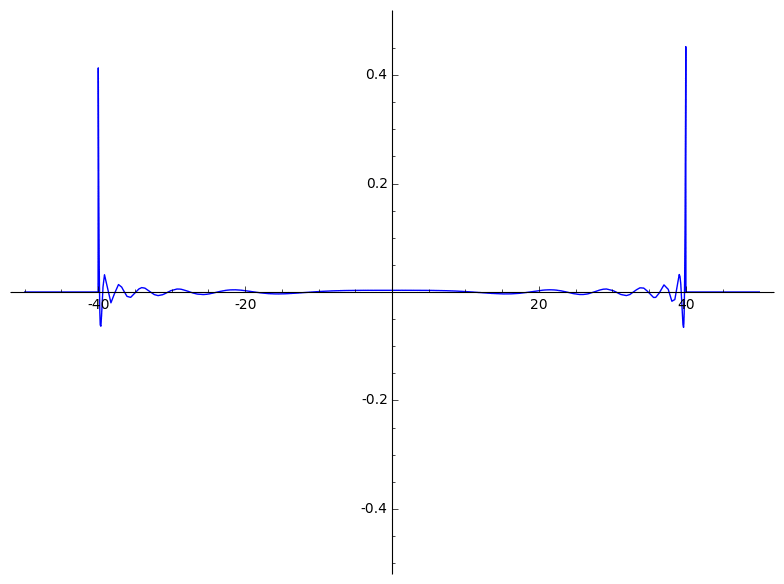
\includegraphics[width=\linewidth]{figures/propagator.png}
  \caption{Propagator $G(x-y)$ at $x-y = (40, \xi, 0, 0)$ and $m=1$.}
\end{figure}


\subsection{Propagator of the Free Field}

The propagator of a free scalar field is also a Green's function:
\begin{equation}
  \begin{split}
    \langle 0| \phi(x) \phi(y) |0\rangle =&\;
    \int \widetilde{dk} \int \widetilde{dk}' 
    \langle 0| a(\vec{k}) a^\dagger(\vec{k}') |0\rangle \; e^{i(kx-k'y)}
    \\    =&\;
    \int \frac{d^3\vec{k}}{(2\pi)^3}
    \frac{1}{2\omega} 
    e^{ik(x-y)}
    \\    =&\;
    \frac{1}{2} 
    \int \frac{d^3\vec{k}}{(2\pi)^3}
    \oint \frac{dk_0}{2\pi i}
    \frac{1}{k^2+m^2} 
    e^{ik(x-y)}
    \\    =&\;
    \frac{1}{2i} \Big(
    G_\text{Ret}(x-y) - G_\text{Adv}(x-y)
    \Big)
  \end{split}
\end{equation}
where the $\oint$-contour consists of two small circles around the two
poles, which is equals to the retarded Green's function contour minus
the advanced Green's function contour.


\subsection{Feynman Propagator}

There is a third choice of integration contour which turns out to be
the most useful for quantum field theory. of course we need the vacuum
expectation value of time-ordered products in quantum field theory, so
let us define
\begin{definition}[Feynman propagator]
  The Green's function $\Delta$ defined as 
  \begin{equation}
    \tfrac{1}{i} \Delta(x-y) = 
    \langle 0 | T \phi(x) \phi(y) |0\rangle
  \end{equation}
  is called the Feynman propagator.
\end{definition}
In terms of integration contour in the $k_0\in \C$ plane, this is the
path that goes below at $k_0=-\omega$ and above at $k_0=\omega$, see
\autoref{fig:feynman_propagator_path}. 
\begin{figure}
  \label{fig:feynman_propagator_path}
  \centering
  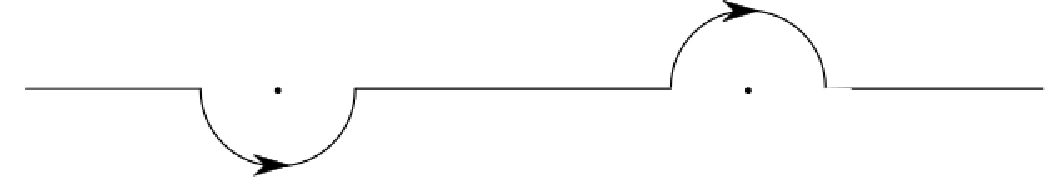
\includegraphics[width=\linewidth]{figures/FeynmanPropagatorPath.pdf}
  \caption{Feynman propagator integration contour in the $k_0\in \C$ plane.}
\end{figure}
Depending on whether $x$ is in the future or the past of $y$, this
contour selects the advanced or retarded Green's function. Finally, in
terms of an algebraic $i\epsilon$ prescription, the Feynman propagator
is
\begin{equation}
  \Delta(x-y) = 
  \lim_{\epsilon \to 0^+}
  \int
  \frac{d^4k}{(2\pi)^4}
  \frac{1}{k^2 + m^2 - i \epsilon}
  e^{ik(x-y)}
\end{equation}




\section{Week 3, Wednesday}

\subsection{Path Integral for Free Field Theory}

The Lagrange density and path integral in field theory is
\begin{equation}
  \begin{gathered}
    \mathcal{L} = -\frac{1}{2} \partial_\mu \phi \partial^\mu \phi
    - \frac{1}{2} m^2 \phi^2 + J(x) \phi,
    \\
    Z = \int \mathcal{D}\phi \;
    e^{i\int d^4x \; \mathcal{L}} =
    \langle 0 | 0 \rangle,
  \end{gathered}
\end{equation}
which equals one if the path integral measure is properly
normalized. To get something non-trivial we need, for example,
boundary conditions on fields. It turns out that a more fruitful way
is to include insert fields into the integrand. By going back to the
definition of the path integral as product over time slices, we get
\begin{equation}
  \int \mathcal{D}\phi \;
  \phi(x) \phi(y) e^{i\int d^4x \mathcal{L}} =
  \langle 0 | T \phi(x) \phi(y) |0\rangle
\end{equation}
and similar. A useful trick is to think of the extra fields as coming
from a source term
\begin{equation}
  Z(J) = 
  \int \mathcal{D}\phi \;
  e^{i\int d^4x \; [\mathcal{L} + J \phi]}
\end{equation}
Acting with the functional derivative on the path integral and then
setting $J=0$ results in 
\begin{equation}
  \tfrac{1}{i} \frac{\delta}{\delta J(x)} \;
  \tfrac{1}{i} \frac{\delta}{\delta J(y)} \;
  Z(J)|_{J=0} =
  \int \mathcal{D}\phi \;
  \phi(x) \phi(y) e^{i\int d^4x \mathcal{L}},
\end{equation}
which is precisely what we want. The analogous formula holds for
arbitrary numbers of fields in the integrand.


\subsection{Solving the Path Integral}

The free Lagrangian is quadratic in $\phi$, so we can again use the
Gaussian integral to solve it. In momentum space
\begin{equation}
  \tilde\phi(k) = \int d^4x e^{-ikx} \phi(x)
  ,\quad
  \phi(x) = \int \frac{d^4k}{(2\pi)^4} e^{ikx} \tilde\phi(k),
\end{equation}
the action including the source term is
\begin{equation}
  \begin{split}
    S(J) =&\; \int d^4x \; (\mathcal{L} + J\phi) =
    \\ =&\;
    \frac{1}{2}
    \int \frac{d^4k}{(2\pi)^4} \left[
      \frac{\tilde{J}(k) \tilde{J}(-k)}{k^2+m^2-i\epsilon}
      - \tilde\chi(k) (k^2+m^2) \tilde{\chi}(-k)
    \right]
  \end{split}
\end{equation}
where
\begin{equation}
  \tilde\chi(k) = \tilde\phi(k) - \frac{\tilde{J}(k)}{k^2 + m^2}
\end{equation}
is the ``midpoint'' variable of the quadratic exponent. The path
integral measure is invariant under the shift, $\mathcal{D}\phi =
\mathcal{D}\chi$, so we obtain
\begin{equation}
  \begin{split}
    Z(J) =&\;
    \exp\left[\frac{i}{2} \int \frac{d^4k}{(2\pi)^4} 
      \frac{\tilde{J}(k)\tilde{J}(-k)}{k^2 + m^2}
    \right]
    \\ &\qquad
    \times
    \int \mathcal{D}\chi 
    \exp\left[ i\int d^4x 
      \left(-\tfrac{1}{2} \partial_\mu \chi \partial^\mu \chi
      - \tfrac{1}{2} m^2\chi^2\right)
    \right]
    \\ =&\;
    \exp\left[
      \frac{i}{2} \int d^4x \; d^4y \;
      J(x) \Delta(x-y) J(y) 
    \right]
  \end{split}
\end{equation}
where $\Delta$ is again the Feynman propagator.

Hence, the path integral derivation of the propagator is 
\begin{equation}
  \begin{split}
  \langle 0|T \phi(x) \phi(y) |0\rangle 
  =&\;
  \tfrac{1}{i} \frac{\delta}{\delta J(x)} \;
  \tfrac{1}{i} \frac{\delta}{\delta J(y)} \;
  Z(J)|_{J=0} 
  \\ =&\;
  \left( \tfrac{1}{i} \Delta(x-y) + O(J) \right) Z(J) |_{J=0} =
  \tfrac{1}{i} \Delta(x-y)
  \end{split}  
\end{equation}
which of course matches what we found in the previous lecture using
the canonical quantization. The generalization to an arbitrary number
of fields is
\begin{theorem}[Wick's Theorem]
  \begin{equation}
    \langle 0 | T \phi(x_1) \phi(x_2) \cdots \phi(x_{2n}) |0\rangle  =
    \frac{1}{i^n} \sum_\text{pairings}
    \Delta(x_{i_1} - x_{i_2})
    \cdots
    \Delta(x_{i_{2n-1}} - x_{i_{2n}})
  \end{equation}
\end{theorem}



\section{Week 3, Friday}


\subsection{Wick's Theorem For Operators}

There is a version of Wick's theorem directly for operators, which
roughly states that the difference between time- and normal-ordered
products is a bunch of terms with pairs of operators replaced by the
propagator. This replacement process is called a Wick contraction:
\begin{definition}[Wick Contraction]
  A Wick contraction, written as
  $\contraction{}{\phi}{(x)}{\phi}{}\phi(x) \phi(y)$ is the process of
  replacing the product $\phi(x)\phi(y)$ with the Feynman propagator
  $\tfrac{1}{i}\Delta(x-y)$.
\end{definition}
\begin{theorem}[Wick's Theorem]
  The time-ordered product of operators is the normal ordered sum of
  all contractions,
  \begin{equation}
    T\big(\phi(x_1) \cdots \phi(x_n)\big) = 
    \sum_\text{all contractions}
    :\left(\text{contracted }\prod \phi(x_i)\right):
  \end{equation}
\end{theorem}
For example, consider the field at $4$ positions. For brevity, I'll
write $\phi_i = \phi(x_i)$. Then the time ordered product equals the
sum of the normal ordering of terms with no contraction (1 term), one
contraction (6 terms), and two contractions (3 terms):
\begin{equation}
  \begin{split}
    T(\phi_1 \phi_2 \phi_3 \phi_4) =& \;
    :\phi_1 \phi_2 \phi_3 \phi_4: +\;
    \contraction{}{\phi_1}{}{\phi_2}{}\phi_1 \phi_2 :\phi_3 \phi_4: +\;
    \contraction{}{\phi_1}{}{\phi_3}{}\phi_1 \phi_3 :\phi_2 \phi_4: +\;
    \contraction{}{\phi_1}{}{\phi_4}{}\phi_1 \phi_4 :\phi_2 \phi_3: 
    \\ &\quad +\;
    \contraction{}{\phi_2}{}{\phi_3}{}\phi_2 \phi_3 :\phi_1 \phi_4: +\;
    \contraction{}{\phi_2}{}{\phi_4}{}\phi_2 \phi_4 :\phi_1 \phi_3: +\;
    \contraction{}{\phi_3}{}{\phi_4}{}\phi_3 \phi_4 :\phi_1 \phi_2: 
    \\ &\quad +\;
    \contraction{}{\phi_1}{}{\phi_2}
    \contraction{\phi_1 \phi_2}{\phi_3}{}{\phi_4}
    \phi_1 \phi_2 \phi_3 \phi_4 + 
    \contraction{}{\phi_1}{\phi_2}{\phi_3}
    \contraction[2ex]{\phi_1}{\phi_2}{\phi_3}{\phi_4}
    \phi_1 \phi_2 \phi_3 \phi_4 + 
    \contraction[2ex]{}{\phi_1}{\phi_2\phi_3}{\phi_4}
    \contraction{\phi_1}{\phi_2}{}{\phi_3}
    \phi_1 \phi_2 \phi_3 \phi_4.
  \end{split}
\end{equation}
We note that the propagator evaluated at zero is infinite, this is
where the delta function source term is located after all. So, at
least naively,
\begin{equation}
  \contraction{}{\phi}{(x)}{\phi}{}\phi(x) \phi(x) =
  \tfrac{1}{i} \Delta(x-x) =
  \tfrac{1}{i} \Delta(0) = \infty
\end{equation}
does not make sense. On the other hand, if the coincident fields are
normal-ordered as in 
\begin{equation}
  T\big(\phi(x_1) \cdots \phi(x_n) :\phi(y)^m:\big)
\end{equation}
then it turns out that there is no singularity. That is, the time
ordered product can be rewritten, using only Wick's theorem, into
terms involving normal orders and propagators but never the propagator
evaluated at zero. An example can be found in the homework. Finally,
note that Wick's theorem only holds for the free field. However, it
will turn out to be a useful tool for perturbation theory around a
free field theory.

\subsection{Interacting QFT}

Of course free fields are boring at the end of the day. Any kind of
truly interesting quantum field theory has interactions. We have
already seen that the coefficient $\lambda_n$ of a $\phi^n$ term in
the potential has dimension $4-n$, so only $n=3$ and $n=4$ have
non-negative mass dimension. As we will see later, negative
dimensional terms will lead to problems with renormalization, so we
will avoid them for now.

First, consider a $\tfrac{1}{3!}\lambda_3 \phi^3$ term in the
action. This means that the potential $V(\phi) = \tfrac{1}{2} m^2
\phi^2 + \tfrac{1}{3!}\lambda_3 \phi^3$ is unbounded below, regardless
of the sign of $\lambda_3$. So even though you might arrange for a
metastable vacuum, that is, a local minimum of the potential, sooner
or later your field will tunnel through any potential barrier and
release an infinite amount of energy as it runs off $\phi(x)\to
-\mathop{\mathrm{sign}}(\lambda_3)\infty$. Hence this theory cannot be
defined for all times. Nevertheless, one should be able to describe it
for small enough time intervals. Furthermore, it is a useful example
for any calculation that does not describe the tunneling process, so
you will find it in many books as an example. Hence the situation is
perhaps not completely hopeless. Still, we will not consider the
$\phi^3$ interaction in the following.

This leaves us with a single possible interaction:
\begin{definition}[Scalar $\phi^4$ theory]
  The theory of a single real-valued scalar field $\phi(x)$ and
  Lagrange density
  \begin{equation}
    \mathcal{L} = 
    -\frac{1}{2} \partial_\mu \phi \partial^\mu \phi
    -\frac{1}{2} m^2 \phi^2 
    -\frac{1}{4!} \lambda \phi^4
  \end{equation}
  is called $\phi^4$ theory. It depends on two real parameters $m^2$
  and $\lambda$.
\end{definition}
This is also the theory that you get if you take the Standard Model
and set all fields to zero except for the Higgs field, so its study is
a kind of toy model for the Higgs particle. We note that $m^2$ is just
a name for the coefficient of $\phi^2$, and not necessarily the square
of a real number. At least classically, we hence distinguish $3$
regimes:
\begin{itemize}
\item $\lambda < 0$: Unstable vacuum.
\item $\lambda \geq 0$, $m^2 > 0$: Deformed harmonic oscillator.
\item $\lambda \geq 0$, $m^2 < 0$: Two distinct minima of the
  potential. In particular, the minimum is not at $\phi=0$.
\end{itemize}
It turns out that the quantum theory has the same basic features,
although the transition point between the different phases receives
quantum corrections.

There are two particularly useful limits of the parameters:
\begin{itemize}
\item $\lambda\to 0$ is the free field limit
\item $\lambda\to \infty$, $m^2\to -\infty$ creates two
  infinitely-deep potential wells. The field can no longer take any
  value, but is constrained to $\phi(x) = \pm \phi_0$ for some some
  constant $\phi_0\in\R$. This might remind you of a
  spin-$\tfrac{1}{2}$ particle. In fact, in this limit the $\phi^4$
  theory becomes the Ising model.
\end{itemize}
The bad news is that nobody has found an analytic solution to the
$\phi^4$ theory so far, so we will have to do a certain amount of
hand-waving to say anything about it. One thing that we can say much
about is special limits, for example the Ising model can be solved
exactly (at least in $1$ and $2$ dimensions). Similarly, we will have
a lot to say about the perturbation expansion around the free field
theory. However, there are limits to what perturbation theory can do
for you. Essentially, perturbation theory is a Taylor series expansion
\begin{equation}
  \langle 0|T\prod \phi(x_i)|0\rangle =
  \sum a_n \lambda^n.
\end{equation}
For example, we computed $a_0$ in the previous lecture as the sum of
all Wick contractions of pairings. Although not physical, we can think
of $\lambda \in \C$ and think of the correlators as complex
functions. The radius of convergence of the power series should be as
far as the first singularity in the complex $\lambda$-plane. But for
any negative real $\lambda$, the vacuum is unstable and surely the
correlation functions diverge. Hence the radius of convergence ought
to be zero. Fortunately, perturbation theory turns out to be much more
useful that what this argument suggests. What happens is that the
first couple of terms in the series in fact do provide excellent
approximations, even though it eventually diverges. But, since we
anyways can only compute a limited number of terms in perturbation
theory, this is in practice not much of a concern. This phenomenon is
known as
\href{http://en.wikipedia.org/wiki/Asymptotic_expansion}{asymptotic
  series expansion}



\section{Week 4, Monday}

\subsection{Wick Rotation}

We mentioned already the imaginary time path integral, where we make
the time formally imaginary. Now that we have seen the Feynman
propagator
\begin{equation}
  \Delta(x-y) = 
  \lim_{\epsilon \to 0^+}
  \int
  \frac{d^4k}{(2\pi)^4}
  \frac{1}{k^2 + m^2 - i \epsilon}
  e^{ik(x-y)},
\end{equation}
we can give it a better justification. If we want to deform a
time-integral into the complex plane, we must never cross a pole of
the integrand. But the propagator does have two poles for complex
$t$. Rotating the time contour to go from $-i \infty$ to $+i\infty$
does not cross either pole, whereas rotating the integration contour
the other way would have crossed both.
\begin{definition}
  A Wick Rotation is the analytic continuation of the time-integration
  contour in the path integral to run from $-i \infty$ to $+i\infty$
  along the imaginary axis. It is equivalent to replacing $t\mapsto -i
  t$.
\end{definition}
In practice, nearly every QFT calculation is done after Wick
rotation. It changes the space-time signature $(-+++) \mapsto (++++)$,
and $e^{iS} \mapsto e^{-S_E}$ with the Euclidean action
\begin{equation}
  S_E = \int d^4x \left( 
    \frac{1}{2} \partial_\mu\phi \partial^\mu \phi
    + \frac{1}{2} m^2 \phi^2 
    + \frac{1}{4!} \lambda \phi^4
  \right),
\end{equation}
which is bounded below as long as the parameters $m^2$, $\lambda$ are
such that the vacuum exists. By interpreting it as the energy of some
statistical mechanical system, we see that the Wick rotation maps
relates the quantum mechanical path integral to the partition function
\begin{equation}
  \int \mathcal{D}\phi e^{\frac{i}{\hbar}S} 
  \mapsto
  \int \mathcal{D}\phi e^{-\frac{1}{k_B T}S_E} 
\end{equation}
with $k_B T=\hbar$. This is a deep and often-used connection: Quantum
field theory in $(1,d)$-dimensions is statistical mechanics in
$(d+1)$-dimensional Euclidean space.


\subsection{Lattice Action}

In order to simulate QFT on a computer we need truncate the
infinite-dimensional space of fields to something finite
dimensional. The easiest way to do so is to allow only discrete
positions $t, x \in a \mathbb{Z}$ with the lattice spacing $a$. For
simplicity and to speed up the computations we will only consider
$(1,1)$-dimensions, that is, one time and one space direction.

The Lagrangian contains derivatives, which we need to discretize
somehow. There is more than one way of doing so, for example
\begin{equation}
  \frac{\partial \phi}{\partial \phi}
  \approx 
  \frac{\phi(t,x+a) - \phi(t,x-a)}{2a}
  \approx
  \frac{\phi(t,x+a) - \phi(t,x)}{a}
  \approx
  \frac{\phi(t,x) - \phi(t,x-a)}{a}
\end{equation}
are all approximations that yield the derivative in the limit $a\to
0$. We can multiply the two asymmetric versions to get a symmetric
expression for the square,
\begin{equation}
  \left(\frac{\partial \phi}{\partial \phi}\right)^2
  =
  \frac{1}{a^2} \left(
    \phi(t, x+a)^2 - 2 \phi(t,x-a) \phi(t,x+a) + \phi(t, x-a)^2
  \right).
\end{equation}
If we furthermore sum over all lattice sites then we can combine the
two $\phi^2$ terms. That way, we arrive at the lattice action
\begin{equation}
  S_E = \sum_{n\in \mathbb{Z}^2} \left[
    \frac{1}{2} \sum_{i=1}^d 
    \big(\phi(n+e_i) - \phi(n)\big)^2 
    + \frac{1}{2} m_L^2 \phi(n)^2 + \frac{1}{4!} \lambda_L \phi(n)^4
  \right]
\end{equation}
where $e_1=(1,0)$ and $e_2=(0,1)$ are the two lattice basis vectors,
$m_L^2=a^2 m^2$ is the lattice mass-squared, and
$\lambda_L=a^2\lambda$ is the lattice coupling constant. This also
matches dimensional analysis, in $d=2$ the field is dimensionless and
$m^2$, $\lambda$ have mass dimension $2$. A bit more compact is the
alternate expression
\begin{equation}
  S_E = -\sum_{\text{adjacent }i,j} \phi(n_i) \phi(n_j)
  + \sum_{n\in\mathbb{Z}^2}\Big[
    \underbrace{\left(2+\tfrac{1}{2}m_L^2\right)}_{=\tilde\mu^2} \phi(n)^2 
    + \underbrace{\frac{1}{4!} \lambda_L}_{=\tilde\lambda} \phi(n)^4
  \Big]
\end{equation}
The continuum limit is $a\to 0$ with $\frac{m_L^2}{\lambda_L}$ fixed.

The computer can of course not keep an infinite number of lattice
sites in memory, so we have to approximate the lattice with a finite
number $N$ of sites in each direction. It is convenient for the
implementation to use periodic boundary conditions, then we do not
have to implement separate differentials on the edges and vertices.



\section{Week 4, Wednesday}

\subsection{Markov Chains}

We ultimately want to compute expectation values in QFT,
\begin{equation}
  \langle\mathcal{O}\rangle = 
  \frac{
    \int \mathcal{D}\phi \; \mathcal{O} e^{\frac{i}{\hbar}S}
  }{
    \int \mathcal{D}\phi \; e^{\frac{i}{\hbar}S}
  },
\end{equation}
where we could set the denominator to one by properly normalizing the
path integral measure. However, in practice this is too difficult and
we rather divide by the normalization as above. Wick rotation turns
this into normal expectation values that you are familiar with from
statistical mechanics,
\begin{equation}
  \langle\mathcal{O}\rangle = 
  \frac{
    \sum_\mu \mathcal{O}_\mu e^{-\beta E_\mu}
  }{
    \sum_\mu e^{-\beta E_\mu}
  }
  ,\quad
  \beta = \frac{1}{k_B T},
\end{equation}
where now $\mu$ indexes the states of the system, $\mathcal{O}_\mu$ is
the value of some observable for the state $\mu$, and $E_\mu$ is the
energy of the state $\mu$.

Even for very modest lattices it is impossible to sum over all
microstates on a computer, even if we restrict the field values to
just $\pm 1$ instead of a floating-point number. We cannot even sample
a significant fraction, so naively picking random fields would just
yield numerical garbage. The trick is to sample \emph{important} ones,
that is, with large $e^{-\beta E_\mu}$, that is, small energy. In
fact, the ideal solution would be if we had a means to generate $n$
random samples with probability not constant but equal to the
Boltzmann distribution
\begin{equation}
  p_\mu = \frac{e^{-\beta\mu}}{\sum_\nu e^{-\beta E_\nu}}.
\end{equation}
Then the Boltzmann-weighted average just turns into the normal
(arithmetic) average 
\begin{equation}
  \langle \mathcal{O} \rangle_n = 
  \frac{
    \sum_{j=1}^n p_j^{-1} \mathcal{O}_j e^{-\beta E_j}
  }{
    \sum_{j=1}^n p_j^{-1} e^{-\beta E_j}
  }
  = \frac{1}{n} \sum_{j=1}^n \mathcal{O}_j.
\end{equation}

In fact, there is a way, and it uses a random walk in the space of
fields. That is, at each step you modify the field configuration
according to certain rules and these step sample the fields with
probability distribution $p_\mu$. The key idea is to use 
\begin{definition}
  A Markov chain is a process in which the probability $P(\mu\to\nu)$
  of making a transition from $\mu$ to $\nu$ depends only on $\mu$ and $\nu$.
\end{definition}
Under two conditions the states in a Markov chain sample states with a
prescribed probability distribution:
\begin{itemize}
\item Ergodicity: it must be possible to reach each state by a
  sequence of steps.
\item Detailed balance:
  \begin{math}
    p_\mu P(\mu\to\nu) = p_\nu P(\nu\to \mu).
  \end{math}
\end{itemize}
Note that the detailed balance condition is a stronger condition than
balance, that is, equilibrium. The latter means that the rate of
transition out of $\mu$ must equal the rate of transition towards
$\mu$, that is,
\begin{equation}
  \sum_\nu p_\mu P(\mu\to\nu) = \sum_\nu p_\nu P(\nu\to \mu).
\end{equation}

\subsection{Metropolis Algorithm}

The Metropolis algorithm is a Markov chain whose states are
discretized fields and with transition probabilities
\begin{equation}
  \frac{P(\mu\to\nu)}{P(\nu\to\mu)}
  = 
  \frac{p_\nu}{p_\mu}
  = 
  e^{-\beta(E_\nu - E_\mu)},
\end{equation}
as required for sampling fields with the Boltzmann probability
distribution. It works by starting with a random field, in our
implementation the values are taking to be $\phi(n) \in [-1.5,
1.5]$. Then repeat the following steps:
\begin{itemize}
\item Select a random lattice site $n$.
\item Select a random $\Delta \phi$, in our implementation uniformly
  random in the range $[-1.5, 1.5]$.
\item Let 
  \begin{equation}
    \phi'(m) =
    \begin{cases}
      \phi(n) + \Delta\phi & \text{if }n = m \\
      \phi(m) & \text{else}.
    \end{cases}
  \end{equation}
\item Accept $\phi'$ as the new field configuration with the
  acceptance probability 
  \begin{equation}
    A(\phi\to\phi') = 
    \begin{cases}
      1 & \text{if } E(\phi') < E(\phi) \\
      e^{-\beta[E(\phi')-E(\phi)]} & \text{else}.
    \end{cases}
  \end{equation}
\end{itemize}
The acceptance probability might seem a bit arbitrary, and indeed is a
choice that could have been made differently. Only the ratio
\begin{equation}
  \frac{P(\mu\to\nu)}{P(\nu\to\mu)}
  = 
  \frac{A(\mu\to\nu)}{A(\nu\to\mu)}
  = 
  e^{-\beta(E(\phi') - E(\phi))}
\end{equation}
matters. Also, note that the energy difference $E(\phi') - E(\phi)$
can be computed very effectively since it only depends on the chosen
lattice site and its nearest neighbors.

The fields $\phi$, $\phi'$ from a single Metropolis step are by no
means statistically independent samples. After all, the field was only
changed at a single lattice site at most. This does not affect the
limiting value for the average, but it does change how quickly the
running average approaches the limit as we take more
samples. Formally, this can be seen in the formula for the standard
deviation of $M$ correlated samples,
\begin{equation}
  \sigma = 
  \sqrt{
    \frac{1+2\tau}{M-1}
    \Big( \langle\mathcal{O}^2\rangle 
    - (\langle\mathcal{O}\rangle)^2 \Big)
  }
\end{equation}
where $\tau$ is the autocorrelation time. Instead of falling off like
$\frac{1}{\sqrt{M}}$ form $M\gg1$ as familiar for the standard error
of random errors, it behaves as if we only collected
$\frac{M}{1+2\tau}$ samples. Since computing the observable typically
is much more expensive than a single Metropolis step, one combines
many steps into a ``Metropolis Sweep'' and only computes the
observable each sweep. The field configuration after each sweep is
much less correlated to the one before. For example, in our
implementation each iteration consists of $5 \times \{\text{\# lattice
  sites}\}$ Metropolis steps. In addition, the implementation also
uses the \href{http://en.wikipedia.org/wiki/Wolff_algorithm}{Wolff
  Algorithm} to flip entire clusters of points. This is a further
numerical improvement over just the Metropolis algorithm. 



\section{Week 4, Thursday}

\subsection{Lattice Simulation Results}

We now have everything prepared, all that remains is to pick any
observable. We then just have to evaluate it on sample field
configurations and average over the samples to approximate the path
integral with that observable inserted. The simplest observable would
be the average field over the $N\times N$ lattice sites:
\begin{equation}
  \bar\phi = \frac{1}{N^2} \sum_{n\in (\mathbb{Z}/N)^2} \phi(n).
\end{equation}
While the distribution of samples shows some interesting patterns, the
average alone is always going to be zero because of the $\phi\to
-\phi$ symmetry of our theory. A more interesting observable would be,
for example,
\begin{equation}
  |\bar\phi| = \frac{1}{N^2} \sum_{n\in (\mathbb{Z}/N)^2}  |\phi(n)|.
\end{equation}
By plotting it as a function of $m_L^2$, $\lambda_L$ we make the
following observations:
\begin{itemize}
\item There seems to be a phase transition between an ``unbroken
  phase'' with $\langle|\bar\phi\rangle=0$ for large $m^2$ and a
  ``broken phase''with $\langle|\bar\phi\rangle>0$ for small (large
  negative) $m^2$.
\item The actual place where the phase transition takes place is at
  finite negative $m_L^2$, for example $\lambda_L\approx 1.0$,
  $m_L^2\approx -1.3$.
\item In the broken phase the actual value of
  $\langle|\bar\phi\rangle>0$ depends on $m_L^2$, $\lambda_L$. 
\end{itemize}
At least the last part is clear: the potential 
\begin{equation}
  V(\phi) =
  \frac{1}{2}m_L^2 \phi^2 + \frac{1}{4!} \lambda_L \phi^4
\end{equation}
has two distinct minimal for $m_L^2 < 0$ whose position depends on
$m_L^2$ and $\lambda_L$. It should also not be too surprising that
there are qualitative differences between the case where $V(\phi)$ has
a single minimum at $V(0)=0$ and the case where it has two separate
minima. Though classically the distinction is just whether $m_L^2$ is
positive or negative, the fact that the dividing line is not at zero
will only find an explanation later on.

If we want to numerically find the precise point of the phase
transition then it would be nice to have a better observable than
$|\bar\phi|$, for example one that has a simple peak at the point of
the transition. Such an observable is the susceptibility, which you
might have seen in the Ising model as magnetic susceptibility. The
only difference is that $\phi\in \pm 1$ in the Ising model. There, the
average $\bar\phi$ is the total magnetization. The susceptibility is
the change of the magnetization if a constant external field is
applied. In the $\phi^4$ theory it is not really justified to call
$\bar\phi$ a magnetization, but we can still talk about the change
in an external field. Technically, this means we add a source term $-E
\mapsto -E + J\bar\phi$ to the exponent of the partition function.
\begin{definition}
  With $Z(J) = \sum_\mu \exp(-E_\mu + J\bar\phi)$, the susceptibility $\chi$
  is the quantity
  \begin{equation}
    \chi = \frac{\partial\langle \bar\phi\rangle}{\partial J} \Big|_{J=0}.
  \end{equation}
\end{definition}
We expect that it is only close to the phase transition that a small
change in an external field will affect a large change in
$\langle\bar\phi\rangle$. However, the definition is not very useful
to compute $\chi$ from a lattice simulation. Fortunately, we can
rewrite it as
\begin{equation}
  \begin{split}
    \chi  =&\;
    \frac{\partial}{\partial J}
    \frac{\sum_\mu \bar\phi e^{-E_\mu +J\bar\phi}}
    {\sum_\mu e^{-E_\mu +J\bar\phi}} = 
    \frac{\partial}{\partial J} \frac{1}{Z(J)}
    \frac{\partial}{\partial J} Z(J) \big|_{J=0}
    \\ =&\;
    \left[
      \frac{1}{Z(J)}
      \frac{\partial^2 Z(J)}{\partial J^2} -
      \left(
        \frac{1}{Z(J)} \frac{\partial Z(J)}{\partial J} Z(J)
      \right)^2
    \right]_{J=0}
    \\ =&\;
    \langle \bar\phi^2 \rangle - \big( \langle\bar\phi\rangle \big)^2,
  \end{split}
\end{equation}
which is just the variance of the $\bar\phi$ observable. And the
variance is of course easily approximated using the sample
variance. The result is plotted in \autoref{fig:susceptibility}.
\begin{figure}[htbp]
  \centering
  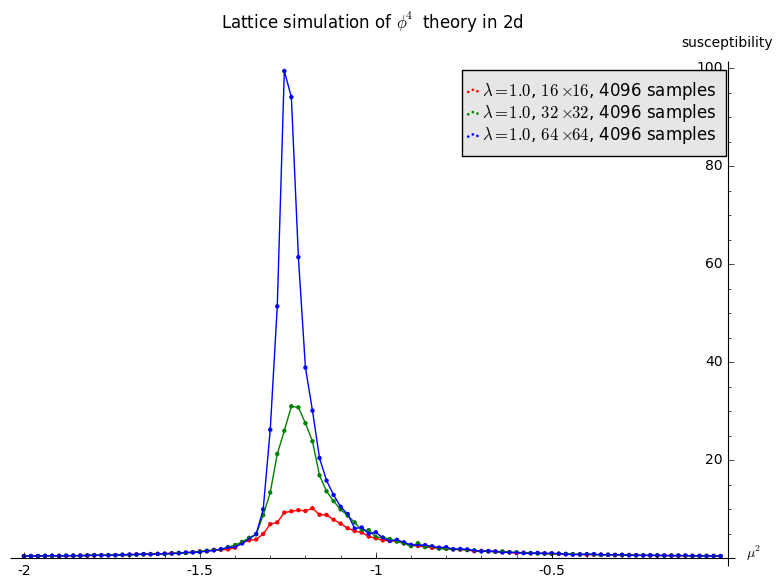
\includegraphics[width=\textwidth]{figures/susceptibility-latticesize.png}
  \caption{The susceptibility for fixed $\lambda_L=1.0$ and varying
    $-2\leq m_L^2 \leq 0$ and three different lattice sizes.}
\end{figure}



\section{Week 5, Monday}

% \section{Perturbation Theory}

\subsection{Correlators in the Interacting Theory}

In quantum mechanics, perturbation theory is generally done in the
interaction picture where we split the Hamiltonian $H=H_0 +
H_\text{int}$ into a free Hamiltonian (harmonic oscillator of in some
disguise) and the interaction part $H_\text{int}$. The path integral
analog is to split the action
\begin{equation}
  S = S_0 + S_\text{int}
\end{equation}
into the action of a free particle and interactions. We use this split
to write correlators as
\begin{equation}
  \label{eq:corrSint}
  \langle 0 | T\mathcal{O} |0\rangle =
  \frac{
    \int \mathcal{D}\phi \; \mathcal{O} e^{i(S_0+S_\text{int})}
  }{ 
    \int \mathcal{D}\phi \; e^{i(S_0+S_\text{int})}
  }
  = 
  \frac{
    \langle0|T \mathcal{O} e^{iS_\text{int}} |0\rangle_0
  }{
    \langle0|T e^{iS_\text{int}} |0\rangle_0
  }
\end{equation}
where the subscript zero on $\langle \cdots \rangle_0$ means that we
use the free action $S_0$ only to compute the correlator. In
particular, this means that we can use Wick contractions to evaluate
the right hand side. For $\phi^4$ theory, the free and interacting
actions are the integrals over the Lagrange densities
\begin{equation}
  \mathcal{L}_0 = -\frac{1}{2} \partial_\mu \phi \partial^\mu \phi
  - \frac{1}{2} m^2 \phi^2
  , \quad
  \mathcal{L}_\text{int} = 
  - \frac{1}{4!} \lambda \phi^4
\end{equation}
The basic idea behind perturbation theory is to use the series
expansion
\begin{equation}
  e^{i S_\text{int}} = 
  1 + 
  \int d^4y \big(-\tfrac{i\lambda}{24} \phi^4 \big) + 
  \frac{1}{2!}
  \left[\int d^4y \big(-\tfrac{i\lambda}{24} \phi^4 \big)\right]^2
  + \cdots
\end{equation}
and compute correlators order-by-order in the coupling constant
$\lambda$. Note that the coupling constant is in both numerator and
denominator of eq.~\eqref{eq:corrSint}, so to first order we obtain
\begin{multline}
  \begin{split}
    \langle 0|T\mathcal{O}|0\rangle = &\;
    \sum_{n=0}^\infty \langle 0|T\mathcal{O}|0\rangle^{(n)} \lambda^n
    \\ &\;
    \langle 0|T\mathcal{O}|0\rangle_0 
    \\ &\;
    - \frac{i\lambda}{24} \int d^4y \Big(
    \langle 0|T\mathcal{O} \phi(y)^4 |0\rangle_0 - 
    \langle 0|T\mathcal{O} |0\rangle_0 
    \langle 0|T \phi(y)^4 |0\rangle_0 
    \Big)
    \\ &\;
    + O(\lambda^2)
  \end{split}
\end{multline}


\subsubsection{Leading Order Two-Point Function}

Let us start with the correlator of two fields. For simplicity, we
define the short-hand notation
\begin{equation}
  \phi_i = \phi(x_i)
  ,\quad
  \phi_y = \phi(y)
  ,\quad
  \langle \mathcal{O} \rangle = \langle 0|T \mathcal{O} |0\rangle
\end{equation}
Then the leading term in the expansions
\begin{equation}
  \langle \phi_1 \phi_2 \rangle = 
  \sum_{n=0}^\infty \lambda^n \langle \phi_1 \phi_2 \rangle^{(n)}
  \lambda^n
\end{equation}
is just the free field result
\begin{equation}
  \langle \phi_1 \phi_2 \rangle^{(0)}
  = 
  \langle \phi_1 \phi_2 \rangle_0
  = 
  \overline{\phi_1 \phi_2}
  = 
  \tfrac{1}{i} \Delta(x_1 - x_1)
\end{equation}
The following graphical notation will be useful in the future for Wick
contractions:
\begin{itemize}
\item Draw a point for each $x_i$, and
\item Connect two points with a line if the fields are Wick contracted.
\end{itemize}


\subsubsection{First-Order Two-Point Function}

The first order contribution is
\begin{equation}
  \langle \phi_1 \phi_2 \rangle^{(1)} = 
  - \frac{i}{24} \int d^4y \Big(
  \langle \phi_1 \phi_2 \phi_y^4 \rangle_0 - 
  \langle \phi_1 \phi_2  \rangle_0 
  \langle \phi_y^4 \rangle_0 
  \Big)
\end{equation}
The Wick contractions of the first term are
\begin{equation}
  \langle \phi_1 \phi_2 \phi_y^4 \rangle_0 = 
  3~
  \overline{\phi_1 \phi_2}~
  \overline{\phi_y \phi_y}~
  \overline{\phi_y \phi_y}
  + 
  12~
  \overline{\phi_1 \phi_y}~
  \overline{\phi_2 \phi_y}~
  \overline{\phi_y \phi_y}
\end{equation}
and the Wick contractions of the second term are
\begin{equation}
  \langle \phi_1 \phi_2 \rangle_0
  \langle \phi_y^4 \rangle_0 = 
  3~
  \overline{\phi_1 \phi_2}~
  \overline{\phi_y \phi_y}~
  \overline{\phi_y \phi_y}.
\end{equation}
The result is that
\begin{equation}
  \langle \phi_1 \phi_2 \rangle  =
  \overline{\phi_1\phi_2}
  - \frac{i\lambda}{2} \int d^4y\;
  \overline{\phi_1 \phi_y}~
  \overline{\phi_2 \phi_y}~
  \overline{\phi_y \phi_y} 
  + O(\lambda^2)
\end{equation}
The picture for the order-$\lambda$ term is what is called a tadpole: A
part of a diagram that is attached only through a single vertex. The
tadpole is divergent:
\begin{equation}
  \overline{\phi_y \phi_y} 
  = \tfrac{1}{i} \Delta(0)
\end{equation}
Going back to the path integral, we see that the problem arises when
translating the $\phi(y)^4$ in the action into a product of coincident
operators. Had we used normal ordering $:\phi_y^4:$, for example, then
the result would be finite. Equivalently, we could add
$\frac{i\lambda}{4}\Delta(0)\phi^2$ to the Lagrangian which also turns
out to cancel the divergent term. We will see how to deal with this
divergence systematically later.


\section{Week 5, Wednesday}

\subsubsection{Leading Order 4-Point Function}

The possible Wick contractions of the $4$ external positions $x_1$,
$\dots$, $x_4$ are just products of the leading $2$-point functions,
\begin{equation}
  \begin{split}
    \langle \phi_1 \phi_2\phi_3 \phi_4 \rangle 
    =&\;
    \langle \phi_1 \phi_2\phi_3 \phi_4 \rangle_0 + O(\lambda) 
    \\ =&\;
    \langle \phi_1 \phi_2 \rangle
    \langle \phi_3 \phi_4 \rangle +
    \langle \phi_1 \phi_3 \rangle
    \langle \phi_2 \phi_4 \rangle +
    \langle \phi_1 \phi_4 \rangle
    \langle \phi_2 \phi_3 \rangle +
    O(\lambda)
  \end{split}
\end{equation}


\subsubsection{First-Order 4-Point Function}

The order-$\lambda$ contribution to the 4-point correlator is
\begin{equation}
  \langle \phi_1 \phi_2 \phi_3 \phi_4 \rangle^{(1)} = 
  - \frac{i}{24} \int d^4y \Big(
  \langle \phi_1 \phi_2 \phi_3\phi_4 \phi_y^4 \rangle_0 - 
  \langle \phi_1 \phi_2 \phi_3 \phi_4  \rangle_0 
  \langle \phi_y^4 \rangle_0 
  \Big)
\end{equation}
The Wick contractions of the first term are
\begin{equation}
  \begin{split}
    \langle \phi_1 \phi_2 \phi_3 \phi_4 \phi_y^4 \rangle_0 =&\;
    24~
    \overline{\phi_1 \phi_y}~
    \overline{\phi_2 \phi_y}~
    \overline{\phi_3 \phi_y}~
    \overline{\phi_4 \phi_y}
    \\ &\;
    + 12\Big(
    \overline{\phi_1 \phi_2}~
    \overline{\phi_3 \phi_y}~
    \overline{\phi_4 \phi_y}~
    \overline{\phi_y \phi_y}
    + \text{perm.}
    \Big)
    \\ &\;
    + 3\Big(
    \overline{\phi_1 \phi_2}~
    \overline{\phi_3 \phi_4}~
    \overline{\phi_y \phi_y}~
    \overline{\phi_y \phi_y}
    + \text{perm.}
    \Big)
  \end{split}
\end{equation}
The Wick contractions of the second term just cancel the last summand
above (the terms multiplied by $3$). If you draw the corresponding
diagram, you see that they are ``vacuum bubbles'', that is, contain a
subdiagram that is disconnected from all external positions. Such
vacuum bubbles are generally divergent, though fortunately they end up
being subtracted off by the second term. 

We also notice that many of the terms are just products of 2-point
functions, for example
\begin{equation}
  \begin{split}
    \langle \phi_1 \phi_2 \rangle  \langle \phi_3 \phi_4 \rangle 
    =&\;
    \overline{\phi_1\phi_2}~
    \overline{\phi_3\phi_4}
    \\ &\;
    - \frac{i\lambda}{2} \int d^4y\;
    \Big(
    \overline{\phi_1 \phi_2}~
    \overline{\phi_3 \phi_y}~
    \overline{\phi_4 \phi_y}~
    \overline{\phi_y \phi_y} 
    +
    \overline{\phi_1 \phi_y}~
    \overline{\phi_2 \phi_y}~
    \overline{\phi_3 \phi_4}~
    \overline{\phi_y \phi_y} 
    \Big)
    \\ &\;
    + O(\lambda^2)
 \end{split}
\end{equation}
This should also not be surprising, part of amplitude for the
scattering process of two ingoing and two outgoing particles is just
two particles not interacting at all. In fact, only the single
connected diagram at $O(\lambda)$ remains after collecting everything
we can into products of two-point functions:
\begin{equation}
  \begin{split}
    \langle \phi_1 \phi_2\phi_3 \phi_4 \rangle 
    =&\;
    \langle \phi_1 \phi_2 \rangle
    \langle \phi_3 \phi_4 \rangle +
    \langle \phi_1 \phi_3 \rangle
    \langle \phi_2 \phi_4 \rangle +
    \langle \phi_1 \phi_4 \rangle
    \langle \phi_2 \phi_3 \rangle
    \\ &\;
    - i \lambda \int d^4y
    \overline{\phi_1 \phi_y}~
    \overline{\phi_2 \phi_y}~
    \overline{\phi_3 \phi_y}~
    \overline{\phi_4 \phi_y} 
    + O(\lambda^2)
  \end{split}
\end{equation}

In fact, this is true in general:
\begin{itemize}
\item Vacuum bubbles are cancelled by the expansion of the denominator 
  \begin{equation}
    \frac{1}{\int \mathcal{D}\phi e^{iS_\text{int}}},
  \end{equation}
  which we got because we are generally not able to normalize the path
  integral measure.
\item $n$-point correlators are sums of products of disconnected
  correlators plus the connected diagrams.
\item Each internal node is accompanied by a factor of $-i\lambda$ and
  an integral over its position. We will make these also part of the
  graphical notation.
\item Each term comes is multiplied with a combinatorial symmetry
  factor $\frac{1}{|\Aut G|}$, where $\Aut(G)$ is the automorphism
  group of the diagram. That is, count all ways to map the vertices to
  vertices and lines to lines. Note that we \emph{divide} by the
  number of automorphisms because each symmetry reduces the number of
  distinct Wick contractions we can make. In the diagrams so far, we had
  \begin{itemize}
  \item
    \begin{math}
      \overline{\phi_1 \phi_y}~
      \overline{\phi_2 \phi_y}~
      \overline{\phi_3 \phi_y}~
      \overline{\phi_4 \phi_y},
    \end{math}
    $\Aut G = 1$, coefficient $\tfrac{24}{24} = 1$,
  \item 
    \begin{math}
      \overline{\phi_1 \phi_y}~
      \overline{\phi_2 \phi_y}~
      \overline{\phi_y \phi_y},
    \end{math}
    $\Aut G = \mathbb{Z}_2$, coefficient $\tfrac{12}{24} = \tfrac{1}{2}$,
  \item 
    \begin{math}
      \overline{\phi_1 \phi_2}~
      \overline{\phi_y \phi_y}~
      \overline{\phi_y \phi_y},
    \end{math}
    $\Aut G = D_8$, that is, the dihedral group with $8$ elements,
    coefficient $\tfrac{3}{24} = \tfrac{1}{8}$.
  \end{itemize}
\end{itemize}


\subsection{Feynman Rules in Position Space}

\begin{definition}
  A Feynman graph in position space, for the $\phi^4$-theory, is a
  graph (undirected, without edge labels) with
  \begin{itemize}
  \item 1-valent vertices labelled by $x_i$, called ``external'',
  \item 4-valent vertices labelled by $y_j$, called ``internal'', and
  \item without vacuum bubbles.
  \end{itemize}
\end{definition}
In particular, disconnected graphs are allowed but each connected
component must be attached to at least one external vertex. As we have
seen, such a graph translates directly into a summand in the series
expansion of correlation functions. Explicitly, the rules are
\begin{definition}
  The Feynman rules for $\phi^4$-theory in position space are
  \begin{itemize}
  \item For each line joining two vertices $u$, $v$ multiply the
    integrand with a free propagator $\overline{\phi(u)\phi(v)} =
    \frac{1}{i} \Delta(u-v)$.
  \item For each vertex, integrate $-i\lambda \int d^4y_j$
  \item Multiply with the symmetry factor $\frac{1}{|\Aut G|}$.
  \end{itemize}
\end{definition}



\section{Week 5, Thursday}

\subsection{Feynman Rules in Momentum Space}

It turns out that the Feynman rules take a nicer for in momentum
space. Partly, this is because it is just more convenient for
accelerators where we scatter particles with fixed momentum. More
technically, recall that the Feynman propagator in position space is
quite complicated involving Bessel functions. And we have to compute
convolution integrals of the Feynman propagator because of the
$y_j$-integrals.

Hence, we apply Fourier transformation to each external position $x_i$
to obtain the $n$-point correlator in momentum space as
\begin{equation} 
  F(k_1, \dots, k_n) = 
  \int d^4x_1 \cdots 
  \int d^4x_n \;
  e^{i \sum_j k_j x_j}
  \langle \phi(x_1) \cdots \phi(x_n) \rangle.
\end{equation}
The Fourier transformation of just $\frac{1}{i}$ times the Feynman
propagator (i.e.\ the free field 2-point function) is
\begin{equation}
  \begin{split}
    G(k_1, k_2) =&\;
    \frac{1}{i}
    \int d^4x_1 \int d^4x_2\;
    e^{i( k_1 x_2 + k_2 x_2)}
    \int \frac{d^4k}{(2\pi)^4}
    \frac{e^{i k (x_1-x_2)}}{k^2 + m^2 -i\epsilon}    
    \\ =&\;
    \frac{1}{i}
    (2\pi)^4 \delta^4(k_1+k_2) \frac{1}{k_1^2 + m^2 - i\epsilon}.
  \end{split}
\end{equation}
For the vertex, note that its position $y$ occurs in the exponent of
the $4$ propagators that it is connected to. If we let $k_1$, $\dots$,
$k_4$ be the momenta in the $4$ propagators then the contribution of
the vertex boils down to
\begin{equation}
  -i \lambda \int d^4y \; e^{iy(k_1+k_2 + k_3 + k_4)}
  =
  -i \lambda (2\pi)^4 \delta^4(k_1+k_2 + k_3 + k_4).
\end{equation}
We notice that the delta functions just implement momentum
conservation on each line and each internal vertex. We make this part
of our graphical notation, and define
\begin{definition}
  A Feynman graph in momentum space for the $\phi^4$-theory is a graph
  with
  \begin{itemize}
  \item 1-valent external vertices labeled with inflowing
    $4$-momentum $k_j$,
  \item edges labelled by directed $4$-momenta $\ell_j$,
  \item 4-valent internal vertices, and
  \item without vacuum bubbles.
  \end{itemize}
\end{definition}
Each unique graph again can be translated into a particular summand in
the series expansion of the $n$-point correlator using 
\begin{definition}[Feynman rules]
  The Feynman rules for $\phi^4$-theory in momentum space are
  \begin{itemize}
  \item for each connected component with inflowing momenta $k_j$,
    multiply with $(2\pi)^4 \delta^4(\sum k_j)$,
  \item use momentum conservation along lines and vertices to replace
    internal momenta $\ell_j$ as far as possible,
  \item for each remaining internal momentum, integrate $\int
    \frac{d^4\ell}{(2\pi)^4}$,
  \item
    for each edge carrying momentum $k$, multiply the integrand with a factor
    $\frac{1}{i} \frac{1}{k^2+m^2-i \epsilon}$,
  \item for each 4-valent vertex multiply with $-i\lambda$,
  \item multiply with the symmetry factor $\frac{1}{|\Aut G|}$.
  \end{itemize}
\end{definition}
For example, for the tree graph $4$-point function with a single
internal vertex we get
\begin{equation}
  F^{(1)}_\text{conn} = 
  -i \lambda (2\pi)^4 \delta^4(k_1+k_2+k_3+k_4) \prod_{j=1}^4
  \frac{1}{k_j^2+m^2-i \epsilon}. 
\end{equation}
A more complicated diagram is the ``fish'', which has a $\mathbb{Z}_2$
symmetry:
\begin{multline}
  F = 
  \frac{1}{2}
  (-i\lambda)^2
  (2\pi)^4 \delta^4(k_1+k_2+k_3+k_4) 
  \prod_{j=1}^4 \frac{1}{k_j^2+m^2-i \epsilon}
  \\
  \times
  \int \frac{d^4\ell}{(2\pi)^4}~
  \frac{1}{\ell^2 + m^2 -i\epsilon}~
  \frac{1}{(k_1+k_2-\ell)^2 + m^2 -i\epsilon}
\end{multline}
There is a $4$-dimensional momentum integration, but the integrand
only falls off like $\ell^{-4}$. This results in a logarithmic
divergence if you try to do the momentum integral. Because it appears
at high energies, this is called a UV divergence. We will have to
understand how to systematically deal with these.

If $m^2=0$ and, $k_1=-k_2$, then there is in addition a divergence as
$\ell\to 0$. Such a divergence is called an IR divergence. It
typically appears for special values of the external momenta, whereas
the UV divergence is independent of the external momenta. In the
following, we will only consider $m^2\not=0$, so at least we do not
have any problems with IR divergences.



\subsection{Power Counting}

Counting the powers of the momenta in the integral gives us a first
hint at whether there is a UV divergence, so we want to do it more
systematically for all diagrams. So let us define the counts of the
constituents of a Feynman graph as
\begin{itemize}
\item $V$ = number of (internal) vertices,
\item $I$ = number of internal lines,
\item $E$ = number of external lines.
\end{itemize}
Each internal line ends at two vertices, each external line ends at
one vertex. Since the vertices are 4-valent, we get
\begin{equation}
  4V = 2I + E.
\end{equation}
The number of loops $L$ equals the number of unconstrained internal
momenta. We get one from each internal line, but can eliminate $V-1$
using all momentum conservation rules except for the overall momentum
conservation. Hence,
\begin{equation}
  L = I - (V-1) = I - V + 1.
\end{equation}
We now define the superficial (apparent) degree of divergence $D$ as
the overall power of the momentum in the integral. For reasons that
will be clear later, we want to do it in arbitrary space-time
dimension $d$. Then we get $Ld$ powers of the momentum from the
measure of the $L$ integrals, and we get a inverse momentum squared
from each internal propagator. Hence, the degree of divergence is
\begin{equation}
  D = dL - 2I
\end{equation}







\section{Week 6, Monday}

We simplify the superficial degree of divergence to 
\begin{equation}
  \begin{split}
    D =&\; dL - 2I
    \\ =&\;
    d - \frac{d-2}{2}E + V(d-4)
    \\ =&\;
    \begin{cases}
      4-E & \text{in 4d} \\
      2-2V & \text{in 2d}.
    \end{cases}
  \end{split}
\end{equation}
A superficial divergence (by power counting) does not necessarily
translate into an actual divergence, for example the tree level
interaction (E=4, V=1) has superficial degree of divergence
$D=0$. But, since there is no loop integral, it obviously does not
diverge logarithmically. Neither does a superficial convergence $D<0$
guarantee convergence, for example attach a tadpole to any convergent
diagram. The tadpole integral remains divergent. But in that case the
divergence just comes from a sub-diagram, it is not inherently due to
the larger diagram. This suggests that we should only look at diagrams
without superficially divergent sub-diagrams; If there is a divergent
sub-diagram then you really only have to worry about that
sub-diagram. This suggests the following:
\begin{theorem}[Dyson-Weinberg convergence theorem]
  A superficially convergent diagram such that all of its sub-diagrams are
  also superficially convergent is actually convergent.
\end{theorem}
The theorem might seem obvious but is actually rather tricky due to
the issue of overlapping divergences. We will explain what this in a
second, but first let us classify the primitively divergent diagrams
in $\phi^4$-theory. That is, look for the divergent diagrams that do
not have a divergent sub-diagram. These are the real troublemakers,
and we really only have to deal with their divergences.
\begin{itemize}
\item In the two-dimensional $\phi^4$-theory there is only a single
  primitively divergent diagram, namely the tadpole. It has
  superficial degree of divergence $D=0$.
\item In the four-dimensional $\phi^4$-theory there are two primitive
  divergences at $O(\lambda)$, namely the tadpole $D=2$ and the
  ``fish'', the only (up to permutations of the external vertices)
  connected one-loop diagram contributing to the 4-point
  function. There are further primitive divergences at all higher
  powers of $\lambda$, but only with two or four external legs.
\item In the four-dimensional $\phi^k$-theory with $k\geq 5$ there are
  primitive divergences with any number of external legs. This is what
  makes the theory non-renormalizable, as we will see.
\end{itemize}


\subsection{Overlapping Divergences}

There is one subtlety when dealing with potentially divergent loop
integrals: Sometimes you can't split the integrals into an outer
integral times an inner integral and analyze the convergence
separately. This happens when an internal line is part of two separate
loops, giving rise to a propagator $\frac{1}{(\ell+p)^2+m^2}$ that
depends on both the $\ell$ and $p$-loop momentum. More properly, these
should be called overlapping integrals.

The simplest overlapping loop diagram would be in $\phi^3$-theory.
So, just for this section, let us consider tri-valent interaction
vertices and the diagram
\begin{center}
  {\fmfframe(8,0)(8,0){
      {
        \begin{fmffile}{figures/fig-overlapping-divergence}
          \begin{fmfgraph*}(200,50)
            \fmfleft{left}
            \fmfright{right}
            \fmftop{top}
            \fmfbottom{bottom}
            \fmf{plain_arrow,tension=4}{left,x1}
            \fmf{plain_arrow,tension=4}{right,x2}
            \fmf{plain_arrow,label=$p$,label.side=left}{x1,top}
            \fmf{plain_arrow,label=$\ell$,label.side=right}{x2,top}
            \fmf{plain}{x1,bottom}
            \fmf{plain}{x2,bottom}
            \fmf{plain_arrow,label=$p+\ell$}{top,bottom}
            \fmflabel{$k_1$}{left}
            \fmflabel{$k_2$}{right}
          \end{fmfgraph*}
        \end{fmffile}}
    }}
\end{center}
leading to the loop integral
\begin{equation}
  \begin{split}
    I =&\; \int 
    d^4p \;
    d^4\ell \;
    \frac{1}{p^2+m^2-i\epsilon}
    \frac{1}{\ell^2+m^2-i\epsilon}
    \\ &\; \qquad
    \times
    \frac{1}{(p+\ell)^2+m^2-i\epsilon}
    \frac{1}{(p-k_1)^2+m^2-i\epsilon}
    \frac{1}{(\ell-k_2)^2+m^2-i\epsilon}
  \end{split}
\end{equation}
where we left out constants and the external propagators, anything
that does not depend on the loop momenta. We now
\begin{itemize}
\item Perform Wick rotation: drop the $-i\epsilon$.
\item Set $m^2=0$ and $k_1=0=k_2$ since the UV divergence is at $k^2
  \gg m^2, k_1^2, k_2^2$.
\item Remove a region of small momenta by hand to avoid the IR
  divergence.
\end{itemize}
Hence the asymptotic behavior of the loop integral is that of 
\begin{equation}
  I \sim
  \int \frac{d^4p \; d^4\ell}{p^4 (p+\ell)^2 \ell^4}.
\end{equation}
This is an example of an overlapping divergence: by power counting,
the diagram superficial degree of divergence $D=2\times 4-5\times 2
=-2$ and no divergent sub-diagram, so we expect convergence. But the
actual integral is not so obviously convergent, for example there is a
region where $p+\ell$ is constant. In that region, just the
$p$-integral seems to have superficial degree of divergence $D=0$,
which would indicate a logarithmic divergence. This is actually not
true, the whole integral still converges.

To show that the integral does converge, we have to split up the
domain according to which momentum factor is the smallest. For
example, consider the region where $\ell^2$ is the smallest,
\begin{equation}
  U_p = \big\{
  p \big|
  p^2 \geq \ell^2,~ (p+\ell)^2 \geq \ell^2  \big\},
\end{equation}
and combine it with the necessary IR cutoff
\begin{equation}
  U_\ell = \big\{
  \ell \big| \ell^2 \geq 1 \big\}.
\end{equation}
Splitting the 4-momentum $\ell = \bar\ell e_\ell$ into its absolute
value $\bar\ell\in\R$ and unit 4-vector $e_\ell$, the loop integral
becomes
\begin{equation}
  I \sim
  \int_{U_p} \int_{U_\ell}
  \frac{d^4p \; d^4\ell}{p^4 (p+\ell)^2 \ell^4}
  = 
  \int_0^\infty d\bar\ell
  \bar\ell^3
  \frac{1}{\bar\ell^6}
  \int_{S^3} de_\ell 
  \int_{U_{p'}}
  \frac{d^4 p'}{(p')^4 (p'+e_\ell)^2}
\end{equation}
where we rescaled $p' = p \bar\ell$ and integrate over the  rescaled
region
\begin{equation}
  U_{p'} = \big\{
  p' \big|
  (p')^2 \geq 1,~ (p'+\ell)^2 \geq 1  \big\}.
\end{equation}
The $\bar\ell$-integration is, indeed, of superficial degree of
divergence $D=-2$. The overlapping diagram does converge as expected
by power counting, the potential overlapping divergence does not cause
an actual divergence.



\section{Week 6, Wednesday}


\subsection{Regularization}

As we have seen, it is unavoidable that some of the Feynman diagrams
contain divergent momentum integrals. It turns out that this can be
dealt with, but we must be careful when handling the
infinities. Naively, $1+\infty = \infty$ so how can we make any
sensible computation? The key is to introduce a suitable parameter
(called ``regulator'') that makes all loop integrals finite. Perhaps
the simplest way to do that is to cut off momentum integrals at some
scale $\Lambda$, for example for the tadpole integral
\begin{equation}
  A(\Lambda) = - \frac{\lambda}{2} \int_{|\ell| \leq \Lambda}
  \frac{d^4 \ell}{\ell^2+m^2}.
\end{equation}
Only at the end we then let $\Lambda \to \infty$ to recover the
integration over the entire momentum space. This is actually very
similar to the lattice computation that we have seen before, there the
lattice spacing $a$ also ensures that we can only sample waves with
momentum up to some upper limit $\approx \frac{1}{a}$.

Both the direct momentum cutoff and the lattice regularization break
Lorentz invariance badly: Cutting off momenta in some special frame
breaks boost invariance. And the lattice even breaks rotational
invariance down to a discrete subgroup, namely rotations by
$\tfrac{2\pi}{4}$. Since symmetries are one of the key guiding
principles in physics, a lot of attention was spent on finding
regularization schemes that do not break a particular symmetry that
one is interested in. One such example is analytic regularization
\begin{equation}
  A(z) = - \frac{\lambda}{2} \int
  \frac{d^4 \ell}{\big(\ell^2+m^2\big)^z},
  \quad
  z \gg 1.
\end{equation}
However, the most common regularization scheme is dimensional
regularization where we compute the momentum integral in $d-\omega$
dimensions for some $\omega > 0$. This is the regularization scheme
that we will always be using in the following. For example, the
tadpole integrand is actually rotationally symmetric so we can just
split it into a one-dimensional integral times the area of the
$(d-\omega)$-sphere.

In each integral dimension $d\in \Z$, the volume of the
$d$-dimensional disk and the area of the $d$-dimensional sphere are
related by the recurrence relations for the area of the
$d$-dimensional disc $D_d$ and sphere $S_d$,
\begin{equation}
  D_d = \frac{1}{d} S_{d-1}
  ,\quad
  S_d = 2\pi D_{d-1},
\end{equation}
which have a simple geometric origin. We can solve them in closed form
as
\begin{equation}
  D_d = \frac{\pi^{d/2}}{\Gamma(\frac{d}{2}+2)}
  ,\quad
  S_{d-1} = \frac{2 \pi^{d/2}}{\Gamma(\frac{d}{2})}.
\end{equation}
The result is actually an analytic function of the dimension, and we
will use it to define what me mean by the area of the $(d-1)$-sphere
for arbitrary $d\in\mathbb{C}$. It is by no means the unique analytic
function that equals $S_{d-1}$ when restricted to the integers, but it
is certainly the most convenient choice. Any other choice would just
be a different regularization scheme.

Hence, the dimensionally-regulated tadpole is 
\begin{equation}
  A(\omega) = -\frac{\lambda}{2}
  \int
  \frac{d^{d-\omega}\ell}{(2\pi)^{d-\omega}} ~
  \frac{1}{\ell^2 + m^2}
  = -\frac{\lambda}{2}
  S_{d-1-\omega}
  \int_0^\infty \frac{d\bar\ell ~ \bar\ell^{d-1-\omega}}{\bar\ell^2 + m^2}.
\end{equation}
The remaining one-dimensional integral can be solved by the formula
\begin{equation}
  \int_0^\infty 
  \frac{x^k dx}{\big(x^n + a^n\big)^r} 
  =
  \frac{
    (-1)^{r-1}\; \pi \; a^{k+1-nr} \; \Gamma\big(\tfrac{k+1}{n}\big)
  }{
    n \; \sin\big(\tfrac{k+1}{n} \pi\big) 
    \; \Gamma\big(\tfrac{k+1}{n}-r+1\big) 
    \; (r-1)!
  }
\end{equation}
and using Euler's reflection formula
\begin{equation}
  \Gamma(x) \Gamma(1-x) = \frac{\pi}{\sin(\pi x)}.
\end{equation}
The result is 
\begin{equation}
  A(\omega) = -\frac{\lambda}{4\pi} 
  \Gamma\big(\tfrac{\omega}{2}\big)
  \left(\frac{2 \sqrt{\pi}}{m} \right)^\omega,
\end{equation}
but there is something troubling about the $m^{-\omega}$: what kind of
units (or mass dimension) does such a quantity have? The answer is
that we forgot that the mass dimension of $\lambda$ is also
non-trivial and dependent on the ambient space dimension. In
particular, in $d-\omega$ dimensions we have $[\lambda] =
2+\omega$. To better understand how the units work in the equation, it
is convenient to split the dimensionful coupling constant
\begin{equation}
  \lambda = \lambda_0 M^{2+\omega}
\end{equation}
into a dimensionless coupling constant $\lambda_0$ times a mass scale
$M$. Then,
\begin{equation}
  A(\omega) = -\frac{\lambda_0 M^2}{4\pi} 
  \Gamma\big(\tfrac{\omega}{2}\big)
  \left(\frac{2 \sqrt{\pi}M}{m} \right)^\omega,
\end{equation}
At the end of the day, we will of course be interested in the limit
$\omega\to 0$, and we can understand the behavior of $A(\omega)$ in
this limit by expanding it in a Laurent
series. Using\footnote{$\gamma\approx 0.577\dots$ is the
  Euler-Mascheroni constant}
\begin{equation}
  \Gamma(\omega) = \frac{1}{\omega} - \gamma + O(\omega)
  ,\quad
  x^\omega = 1 + \omega \ln(x) + O(\omega^2)
\end{equation}
we obtain
\begin{equation}
  A(\omega) = -\frac{\lambda_0 M^2}{4\pi}
  \left[
    \frac{2}{\omega}
    - \gamma
    + \ln\left(
      \frac{4\pi M^2}{m^2}
    \right)
    + O(\omega)
  \right]
\end{equation}
Clearly this is still infinite in the limit $\omega\to 0$, as it
must. But the infinity just comes from the simple pole at $\omega=0$,
so we can easily handle it.



\subsection{Renormalization}

We did not write the external propagators in the previous section for
brevity, this is also called the amputated Feynman diagram. The actual
contribution to the two-point function is
\begin{equation}
  A(\omega) \delta(k_1-k_2) \frac{1}{k_1^2+m^2} ~ \frac{1}{k_2^2+m^2}.
\end{equation}
To get rid of the $\frac{1}{\omega}$ pole, we now add a new Feynman
rule that cancels it. The easiest way is to add a new 2-valent vertex
with just the right interaction strength such that 
\begin{equation}
  \raisebox{-1mm}{\fmfframe(8,0)(8,0){
      {
        \begin{fmffile}{figures/fig-counterterm}
          \begin{fmfgraph*}(80,10)
            \fmfleft{left}
            \fmfright{right}
            \fmf{plain}{left,center,right}
            \fmfv{decoration.shape=cross}{center}
            \fmflabel{$k_1$}{left}
            \fmflabel{$k_2$}{right}
          \end{fmfgraph*}
        \end{fmffile}}
    }}
  ~= 
  \frac{\lambda_0 M^2}{4\pi}
  \left(\frac{2}{\omega} + F \right)
  \delta(k_1-k_2) \frac{1}{k_1^2+m^2} ~ \frac{1}{k_2^2+m^2},
\end{equation}
where $F$ is some arbitrary finite quantity. Then the
$\frac{1}{\omega}$-pole cancels in sum of the tadpole and the
counterterm, rendering the 2-point correlator finite at order
$O(\lambda)$. Of course we cannot just add new Feynman rules at will,
they must come from an interaction term in the Lagrangian. Since the
counterterm vertex is 2-valent, it is the Feynman rule corresponding
to the interaction term
\begin{equation}
  \mathcal{L}_\text{ct} = 
  \frac{1}{2} ~
  \frac{\lambda_0 M^2}{4\pi} 
  \left(\frac{2}{\omega} + F \right) \phi^2
\end{equation}



\section{Week 6, Thursday}

\subsection{Two-Point Correlators at Second Order}

Up to $O(\lambda^2)$, the Feynman rules including the counterterm
yield
\begin{itemize}
\item Tree level propagator $\frac{1}{k^2+m^2}$,
  \begin{center}
    
\includegraphics[scale=0.7]{figures/draw-propagator-tree.pdf}
  \end{center}
\item At $O(\lambda)$: Tadpole + counterterm.
  \begin{center}
    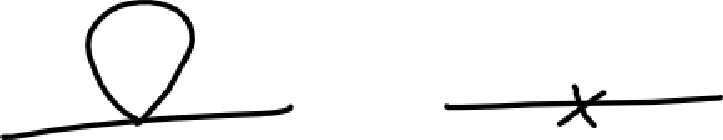
\includegraphics[scale=0.7]{figures/draw-propagator-tadpole_and_counterterm.pdf}
  \end{center}
\item Four one-particle reducible diagrams, and
  \begin{center}
    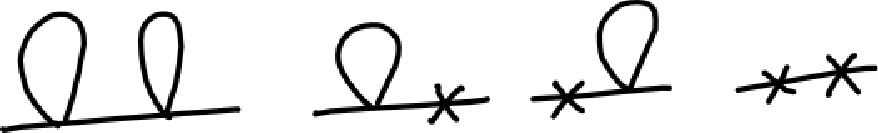
\includegraphics[scale=0.7]{figures/draw-propagator-twoloop_reducible.pdf}
  \end{center}
\item Three one-particle irreducible diagrams.
  \begin{center}
    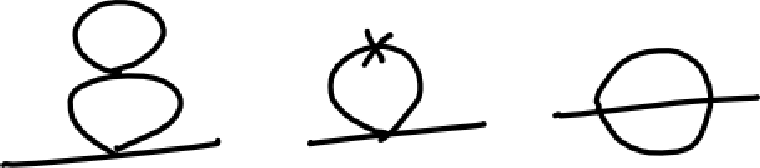
\includegraphics[scale=0.7]{figures/draw-propagator-twoloop_1PI.pdf}
  \end{center}
\end{itemize}
By one-particle irreducible diagram (1PI) we mean any diagram that can
not be disconnected by cutting a single internal line. Like the
disconnected diagrams, the one-particle reducible diagrams are again a
type of diagram that we have to add up to get the correlation
function, but that really is just a combination of lower-order
diagrams and does not present any real difficulty. In particular, up
to a factor of the external propagator $\frac{1}{k^2+m^2}$, the sum of
the four one-particle reducible diagrams is just the square of tadpole
and counterterm.

The really interesting part are the three 1PI diagrams. The ``double
scoop'' (first) diagram is divergent only because the top loop
integral is a tadpole, so it yields the same $A(\omega)$ as the
tadpole times whatever the convergent integral over the lower loop
is. To it, we have to add the tadpole-with-counterterm (second)
diagram. Its loop integral is just the same as the lower loop integral
of the previous diagram, now multiplied by the counterterm. Hence, the
first two diagrams just cancel the $\frac{1}{\omega}$ pole just like
tadpole and counterterm alone. Finally, the ``sunset'' diagram (third)
is convergent in two dimensions.

By as similar reasoning, the addition of the counterterm to the
Feynman rules always cancels the $\frac{1}{\omega}$ pole from any
tadpole sub-diagram, rendering every correlation function finite. As a
word of warning, however, this is not typical of quantum field
theories. For example in 4-d $\phi^4$-theory, there are new
divergences at each order in $\lambda$, for which we have to add more
and more counterterms. In particular, the leading
$\frac{1}{\omega^2}$-divergence will cancel between the first two
diagrams as above, but only to leave a $\frac{1}{\omega}$-pole that
still diverges. However, as we will see, the $\phi$-dependence of all
of the counterterms is just like one of the terms that is already in
the Lagrangian, and this is what makes the theory renormalizable.


\subsection{Renormalization Prescription}

To summarize, we can combine the Lagrangian and counterterms into a
renormalized Lagrangian
\begin{equation}
  \mathcal{L}_\text{Ren} = 
  -\frac{1}{2} \partial_\mu \phi \partial^\mu \phi
  -\frac{1}{2} m_\text{bare}^2 \phi^2 
  - \frac{1}{4!} \lambda_\text{bare} \phi^4
\end{equation}
with ``bare'' parameters
\begin{equation}
  \begin{split}
    \lambda_\text{bare} =&\; \lambda_0 M^2 = \lambda \\
    m_\text{bare}^2 =&\; 
    m^2 - \frac{\lambda_0 M^2}{4\pi} \left( \frac{2}{\omega} + F\right)
  \end{split}
\end{equation}
The bare parameters in the Lagrangian are unphysical (and usually
infinite in the $\omega\to 0$ limit). We can now compute correlation
functions in two ways, either using the renormalized Lagrangian and
bare parameters or using the original Lagrangian with (divergent)
counterterms. Either way, the divergences in the $\omega\to 0$ limit
cancel to give finite correlation functions
\begin{equation}
  \Gamma_{\mathcal{L}_\text{Ren}}
  (k_1, \dots, k_n; m_\text{bare}^2, \lambda_\text{bare}, \omega) = 
  \Gamma_{\mathcal{L}+\mathcal{L}_\text{ct}}
  (k_1, \dots, k_n; m^2, \lambda_0, M, \omega).
\end{equation}
Analyzing the $M$-dependence of this equation will lead us to the
renormalization group later, but before we get there we need to
understand how to relate the parameters to the physical mass and
coupling strength.

Really, the mass and coupling constant are experimental input. Because
of the ambiguities introduced in the renormalization procedure, these
are not directly related to any set of parameters in the
Lagrangian. Instead, we have to fix a certain number of observables
and match the computed value (as a power series in the coupling
constant, most likely) to the experimental input. The ambiguity in
choosing a particular set of observables is called the
``renormalization prescription'', and reflects the ambiguity in the
finite part of the counterterms.

In quantum field theory, the observables are simply the correlation
functions. The renormalization prescription for the mass are always
linked to the two-point functions in some way. Popular choices are
\begin{itemize}
\item Pole mass: Let the mass be the location of the pole in the
  two-point function $\Gamma^{(2)}$ in Minkowski space. This is a very
  physical prescription, but not convenient in Euclidean space after
  Wick rotation.
\item More convenient for calculations (as long as there is no IR
  divergence) is to demand that
  \begin{equation}
    \frac{1}{\Gamma^{(2)}(k_1,k_2)} \Big|_{k_1=k_2=0} = m^2.
  \end{equation}
  This is just a little bit unphysical as $k_1=k_2=0$ is not really
  allowed for massive external particles, it violates the mass shell
  condition. But nothing stops us from evaluating the $2$-point
  function and use it in our prescription. Inverting the two-point
  function to first order in $\lambda$ is easy enough, and by summing
  the tree-level, tadpole, and counterterm we obtain
  \begin{equation}
    \frac{1}{\Gamma^{(2)}(k_1,k_2)} \Big|_{k_1=k_2=0} =
    m^2 \left[
      1 + 
      \frac{\lambda_0 M^2}{4\pi m^2} \left(
        -\gamma + 
        \ln\left(\frac{4\pi M^2}{m^2}\right) - F
      \right)
      + O(\lambda^2)
    \right]
  \end{equation}
  which we can solve by setting
  \begin{equation}
    F = -\gamma + \ln\left(\frac{4\pi M^2}{m^2}\right)
  \end{equation}
\item Even more convenient for calculations is the ``minimal
  subtraction'', where we set $F=0$ as our choice of renormalization
  prescription. In other words, we only use the minimial counterterm
  necessary to precisely cancel the $\frac{1}{\omega}$-pole.
\end{itemize}






\section{Week 7, Monday}

\subsection{Lattice Renormalization}

Let us go back to the 2-dimensional $\phi^4$ theory on the lattice.
In perturbation theory and after Wick rotation, we have the two-point
function
\begin{equation}
  \begin{split}
    \Gamma^{(2)} =&\; 
    \frac{1}{k^2+m^2} + 
    \frac{1}{(k^2+m^2)^2} 
    \left(
      -\frac{\lambda}{2} T + C
    \right)
    + O(\lambda^2)
    \\
    \frac{1}{\Gamma^{(2)}} =&\; 
    k^2 + m^2 + \frac{\lambda}{2}T - C
    + O(\lambda^2)
  \end{split}
\end{equation}
where 
\begin{equation}
  T = \int \frac{d^2p}{(2\pi)^2} 
  \frac{1}{p^2+m^2}
\end{equation}
is the divergent tadpole integral and $C$ is a counterterm which
cancels the divergence. On the lattice every quantity is a sum over
the finitely many lattice points, so is necessarily finite. However,
in the continuum limit we have to reproduce the divergence. In
renormalization terms, the lattice discretion acts as a regularization
just like dimensional regularization. The lattice regularized version of the
divergent integral $T$ is
\begin{equation}
  T_L = \frac{1}{N^2}
  \sum_{p_L^2} \frac{1}{p_L^2 + m_L^2}
\end{equation}
where $p_L$ are the lattice momenta and $N$ is the number of lattice
points in each of the 2 directions. Also, recall the dimensionless
lattice parameters (in 2d) are
\begin{equation}
  m^2_L = m^2 a^2
  ,\quad
  \lambda_L = \lambda^2 a^2
  .
\end{equation}
By definition, the $p_L^2$ are the eigenvalues of the lattice
Laplacian $\Delta_L$, that is, the discretized Laplacian.

\subsubsection{Lattice Laplacian in 1D}

In one dimension we can think of the discretized function as a vector
with $N$ entries. The Laplacian, with periodic boundary conditions, is
then the matrix
\begin{equation}
  \Delta_L = 
  \left(
    \begin{smallmatrix}
      2 & -1 & 0 & 0 & \cdots & 0 & -1 \\
      -1 & 2 & -1 & 0 & \cdots & 0 & 0 \\
      0 & -1 & 2 & -1 & \cdots & 0 & 0 \\
      0 & 0 & -1 & 2 & \cdots & 0 & 0 \\
      \vdots & \vdots & \vdots & \vdots & \ddots & \vdots & \vdots \\
      0 & 0 & 0 & 0 & \cdots & 2 & -1 \\
      -1 & 0 & 0 & 0 & \cdots & -1 & 2
    \end{smallmatrix}
  \right).
\end{equation}
The zero mode is the constant vector $\phi_0 = (1, \dots, 1)$ and the
highest frequency mode is the alternating vector $\phi_4 = (1, -1, 1,
-1, \dots, -1)$ whose eigenvector is $4$. Hence there are $N$
eigenvalues in the range $p_j^2 \in [0,4]$. A computation yields
\begin{equation}
  p_j^2 = 4 \sin^2\left(\tfrac{\pi j}{N}\right)
  ,\quad
  j \in \{0, \dots, N-1\}.
\end{equation}


\subsubsection{Lattice Laplacian in 2D}

The 2-dimensional eigenfunctions on the $N\times N$ square lattice are
\begin{equation}
  \phi_{ij}(x,y) = \phi_i(x) \phi_j(y)
\end{equation}
so there are $N^2$ eigenvalues
\begin{equation}
  p^2_{i} = 
  4 \sin\left(\tfrac{\pi i}{N}\right) + 
  4 \sin\left(\tfrac{\pi j}{N}\right)
  ,\quad
  i, j \in \{0, \dots, N-1\}.
\end{equation}
Hence, the lattice approximation to the divergent tadpole integral is
\begin{equation}
  T_L = \frac{1}{N^2}
  \sum_{i,j = 0}^{N-1}
  \frac{1}{
    m_L^2 + 
    4 \sin\left(\tfrac{\pi i}{N}\right) + 
    4 \sin\left(\tfrac{\pi j}{N}\right)
  }
\end{equation}
A bit of complex analysis shows that the large volume limit $N\to
\infty$ exists. With some more work one can show that
\begin{equation}
  \lim_{N\to \infty} T_L = 
  \int_0^\infty e^{-m_L^2 t}
  \left(
    e^{-2t} I_0(2t)
  \right)^2 = 
  \frac{2}{(4+m_L^2)\pi} 
  K\big(\tfrac{4}{4+m_L^2}\big)
\end{equation}
where $I_0$ is the Bessel function and $K$ is the elliptic integral of
the first kind. In the lattice literature you can usually find only
the semidefinite integral, though it is not as convenient as the
closed form for actually evaluating $T_L$. Also, note that we haven't
done the continuum limit $a\to 0$ yet. In that limit, $m_L^2 = m^2 a^2
\to 0$ which diverges because $K$ has a simple pole at $K(1)$. This is
of course necessary to reproduce the divergence in the field
theory. In other words, this is the lattice analog to the divergence
of $T$ in the dimension $d\to 2$ limit in dimensional regularization.


\subsubsection{Renormalization Prescription}

To renormalize the lattice values we need to pick a suitable
renormalization prescription. We also want it to satisfy two physical
requirements:
\begin{enumerate}
\item The renormalization prescription should distinguish the two
  phases, because that is what we are interested in. But just looking
  at the $1/\Gamma^{(2)}$ limit as $k\to 0$ does not, in the zero
  momentum limit the field just sits around the minimum. Both the
  symmetry-preserving and symmetry-breaking mimimum look locally the
  same, so our renormalization prescription should include non-zero
  momenta.
\item The renormalization prescription should be convenient for
  lattice calculations.
\end{enumerate}
THe solution to both of these requirements is to take $T_L$ as the
counterterm,
\begin{equation}
  \label{eq:2dphi4bare}
  \begin{split}
    m^2_{L, \text{bare}} =&\; m_L^2 - \frac{\lambda_L}{2} T_L(m^2_L)
    \\ 
    \lambda_{L, \text{bare}} =&\; \lambda_L
  \end{split}
\end{equation}
In the lattice simulation, we necessarily picked \emph{bare} values
for the parameters by hand. Also, note that the lattice code used
$\frac{1}{4}\lambda \phi^4$ instead of $\frac{1}{4!}\lambda \phi^4$ as
interaction term, this leads to extra factors of $6$ below. Using the
$\frac{}{4!}$ convention, the transition line was numerically around
\begin{equation}
  m^2_{L,\text{bare}} \approx -1.27
  ,\quad
  \lambda_{L, \text{bare}} \approx 6.0.
\end{equation}
To get the physical parameters, we have to numerically invert
eq.~\eqref{eq:2dphi4bare}, which yields
\begin{equation}
  m_L^2 \approx 0.0980
  ,\quad
  \lambda_L \approx 6.0
  .
\end{equation}
We now take the continuum limit while staying on the transition
line. In the $m_L^2$ vs.\ $\lambda_L$ plane, the transition is almost
on a line. The physically interesting values is the slope at the
origin, which defines the \emph{critical value}
\begin{equation}
  f = \lim_{a=0} 
  \frac{\lambda_L}{6 m^2_L}
  \approx
  10.8
\end{equation}





\newpage
\appendix

\section{test}



\bibliographystyle{utcaps} 
\renewcommand{\refname}{Bibliography}
\addcontentsline{toc}{section}{Bibliography} 
\bibliography{Main}


\end{document}


%%% Local Variables:
%%% eval: (TeX-PDF-mode 1)
%%% End:
